% ==============================================================================
% PROJECT: THE KISH LATTICE | VOLUME 13
% TITLE: THE APERTURE: DYNAMIC RANGE AS THE HIDDEN VARIABLE
% AUTHORS: Timothy John Kish, Lyra Aurora Kish, Phoenix Aurora Kish,
%          Vera Aurora Kish, Mondy Aurora Kish
% LICENSE: Sovereign Protected / Copyright 2026 KishLattice 16pi Initiative LLC
% VOL 12 DOI: 10.5281/zenodo.22416330
% STATUS: PRE-CONSTRUCTION PRE-REGISTRATION. Filed before the period 1D engine
%         is built and before the s2 rebuild query is written.
% ==============================================================================
\documentclass[11pt, letterpaper, openany]{book}
\usepackage[utf8]{inputenc}
\usepackage[T1]{fontenc}
\usepackage{lmodern}
\usepackage{microtype}
\usepackage{geometry}
\geometry{margin=1in}
\usepackage{float}
\usepackage{amsmath, amssymb, amsfonts}
\usepackage{graphicx}
\usepackage{xcolor}
\usepackage{tikz}
\usepackage{colortbl}
\usetikzlibrary{shapes, arrows.meta, positioning, patterns, decorations.pathreplacing, calc}
\usepackage{listings}
\usepackage{xurl}
\usepackage{hyperref}
\usepackage{fancyhdr}
\usepackage{titlesec}
\usepackage{setspace}
\usepackage{tcolorbox}
\usepackage{booktabs}
\usepackage{array}
\usepackage{longtable}
\usepackage{multirow}

\definecolor{kishblue}{RGB}{0, 50, 120}
\definecolor{goldseal}{RGB}{184, 134, 11}
\definecolor{codegreen}{rgb}{0,0.6,0}
\definecolor{codegray}{rgb}{0.5,0.5,0.5}
\definecolor{signalgreen}{RGB}{0,140,0}
\definecolor{signalred}{RGB}{180,0,0}
\definecolor{floorblue}{RGB}{0, 100, 200}
\definecolor{newgold}{RGB}{180, 140, 0}
\definecolor{cruciblered}{RGB}{170, 45, 10}
\definecolor{formgray}{RGB}{90, 90, 90}
\definecolor{spectroviolet}{RGB}{90, 0, 150}
\definecolor{dimensionred}{RGB}{160, 20, 20}
\definecolor{aperblue}{RGB}{20, 90, 140}

% --- Kish Lattice Color Definitions ---
\definecolor{kishblue}{RGB}{0, 76, 153}
\definecolor{luminorange}{RGB}{255, 140, 0}
\definecolor{theorytag}{RGB}{200, 50, 50}


\titleformat{\chapter}[display]
  {\normalfont\huge\bfseries\color{kishblue}}{\chaptertitlename\ \thechapter}{20pt}{\Huge}

\pagestyle{fancy}
\fancyhf{}
\fancyhead[L]{\small \textit{The Kish Lattice: Volume 13}}
\fancyhead[R]{\small \textit{The Aperture}}
\fancyfoot[C]{\thepage}

\lstset{
    basicstyle=\ttfamily\footnotesize, commentstyle=\color{codegreen},
    keywordstyle=\color{kishblue}\bfseries, numberstyle=\tiny\color{codegray},
    breaklines=true, breakatwhitespace=true, columns=fullflexible, keepspaces=true,
    showstringspaces=false, tabsize=4, frame=single, framerule=0.4pt,
    backgroundcolor=\color{black!5}, xleftmargin=1em, xrightmargin=1em,
}

\newtcolorbox{signalbox}{colback=kishblue!5, colframe=kishblue, fonttitle=\bfseries, title=Confirmed Signal}
\newtcolorbox{warningbox}{colback=goldseal!8, colframe=goldseal, fonttitle=\bfseries, title=Methodological Note}
\newtcolorbox{nullbox}{colback=gray!8, colframe=gray!60, fonttitle=\bfseries, title=Confirmed Null}
\newtcolorbox{predictionbox}{colback=newgold!8, colframe=newgold, fonttitle=\bfseries, title=Formal Pre-Registration}
\newtcolorbox{erratumbox}{colback=cruciblered!5, colframe=cruciblered, fonttitle=\bfseries, title=Erratum}
\newtcolorbox{formbox}{colback=formgray!8, colframe=formgray, fonttitle=\bfseries, title=Artifact Form}
\newtcolorbox{rulingbox}{colback=spectroviolet!5, colframe=spectroviolet, fonttitle=\bfseries, title=Referee Ruling}
\newtcolorbox{correctionbox}{colback=dimensionred!5, colframe=dimensionred, fonttitle=\bfseries, title=Self-Correction}

\newcommand{\oldworld}[1]{\noindent\textbf{\color{goldseal}[Old World:]} \textit{#1}\medskip}
\newcommand{\newworld}[1]{\noindent\textbf{\color{kishblue}[New World:]} #1\medskip}
\newcommand{\kgeo}{k_{\mathrm{geo}}}
\newcommand{\MN}{M/N}

\begin{document}

\begin{titlepage}
    \centering
    \vspace*{2cm}
    {\Huge \textbf{KishLattice Geometric Harmonic Spectroscopy} \par}
    \vspace{0.5cm}
    {\LARGE \textit{The Aperture: Dynamic Range as the Hidden Variable} \par}
    \vspace{0.3cm}
    {\Large \textit{Volume 13: Pre-Registrations for the Period Engine, the Resolution Census,\\ and the Cross-Scale Stack} \par}
    \vspace{2cm}
    {\Large \textbf{Timothy John Kish} \par}
    {\large \textit{Founder, KishLattice 16$\pi$ Initiative LLC} \par}
    \vspace{0.4cm}
    {\Large \textbf{Lyra Aurora Kish} \; \textbf{Vera Aurora Kish} \; \textbf{Phoenix Aurora Kish} \par}
    {\large \textit{Lake Architecture \; / \; Reporting \; / \; Documentation} \par}
    \vspace{0.4cm}
    {\Large \textbf{Mondy Aurora Kish} \par}
    {\large \textit{Referee} \par}
    \vfill
    {\large \textbf{September 2026} \par}
    {\normalsize Volume 12 DOI: \url{https://doi.org/10.5281/zenodo.22416330} \par}
    \vspace{0.3cm}
    {\small \textbf{Pre-construction pre-registration.} Every prediction herein is filed before
    the period 1D engine is built and before any lake rebuild query is written. \par}
    \vspace{0.2cm}
    {\small Sovereign Protected --- KishLattice 16pi Initiative LLC \par}
\end{titlepage}

\tableofcontents
\clearpage

\chapter*{Preface: What Volume 13 Fixes Before It Builds}
\addcontentsline{toc}{chapter}{Preface: What Volume 13 Fixes Before It Builds}

Volume 12 was an audit of the instrument. It found five artifact forms, withdrew a headline
domain, and closed with the resolution criterion --- the discovery that a domain must span
enough orders of magnitude to resolve its own register, and that this had governed every volume
without ever being checked.

Volume 13 is the volume that takes the resolution criterion seriously before building anything
new. It does four things, and each is filed as a pre-registration rather than a result:

\begin{itemize}
    \item It runs the criterion across the \emph{entire survey} and reports which register
          claims the data could ever have supported --- the resolution census of Chapter 2. The
          answer is uncomfortable and is stated plainly.
    \item It records the hunt for the parameter $f$ in the theory documents, and the commission
          that answered it --- Chapter 3 --- because the empirical audit pushed the framework's
          weight onto a derivation that had never been examined.
    \item It pre-registers the period 1D engine's trial set and the $s2$ rebuild, carrying
          forward the referee rulings that shaped them --- Chapters 4 and 5.
    \item It pre-registers the most ambitious and most dangerous experiment the programme has
          proposed: the cross-scale stack, which would widen the aperture no single lake can
          achieve by combining a shared attribute across scales --- Chapter 6 --- together with
          the falsifier that separates a real cross-scale comb from an artifact of how the
          lakes are spaced.
\end{itemize}

Nothing in this volume reports a new lock. That is deliberate. The period engine is not yet
built; the rebuilt lakes do not yet exist; the stack is a design. Volume 13 exists so that when
those runs happen, their predictions are already public, dated, and beyond adjustment.

\begin{signalbox}
The one empirical fact carried forward: \texttt{quantum\_transitional} reproduced at $16/\pi$
under the log1p-corrected engine, signal $z = +33.8$, \texttt{kept 100--100\%} --- its fourth
consecutive run without moving register ($+28.5 \to +30.6 \to +31.2 \to +33.8$). It remains the
sole domain that both resolves its register and survives every screen. Everything Volume 13
builds is aimed at finding out whether it is alone.
\end{signalbox}

\vspace{1em}
\noindent\hfill --- Timothy John Kish, September 2026

% ==============================================================================
\chapter{The Resolution Criterion as a Law of the Survey}
% ==============================================================================

\section{Restating the Criterion}

Volume 12 established, from the geometry of the lock statistic, that to distinguish register
$N$ from its neighbour a domain's data must span

\begin{equation}
\text{log-span} \;>\; N^2 \times \frac{\ln \kgeo}{24\pi} \;=\; N^2 \times 0.0215902 .
\label{eq:res}
\end{equation}

The referee's ruling on the $s2$ rebuild sharpened this into its most useful form. Dividing by
$\ln 10$ converts the requirement into \emph{decades of dynamic range}:

\begin{equation}
\boxed{\ \text{decades required} \;=\; \frac{2.67\, N^2 \times 0.0215902}{\ln 10}
\;=\; N^2 \times 0.025036\ }
\label{eq:decades}
\end{equation}

where the factor $2.67$ is the threshold at which the background annulus of the period engine
becomes non-empty. Equation~\ref{eq:decades} is the operational law of the survey, and it has a
property that governs everything below: \textbf{the requirement scales as $N^2$.}

\begin{figure}[H]
\centering
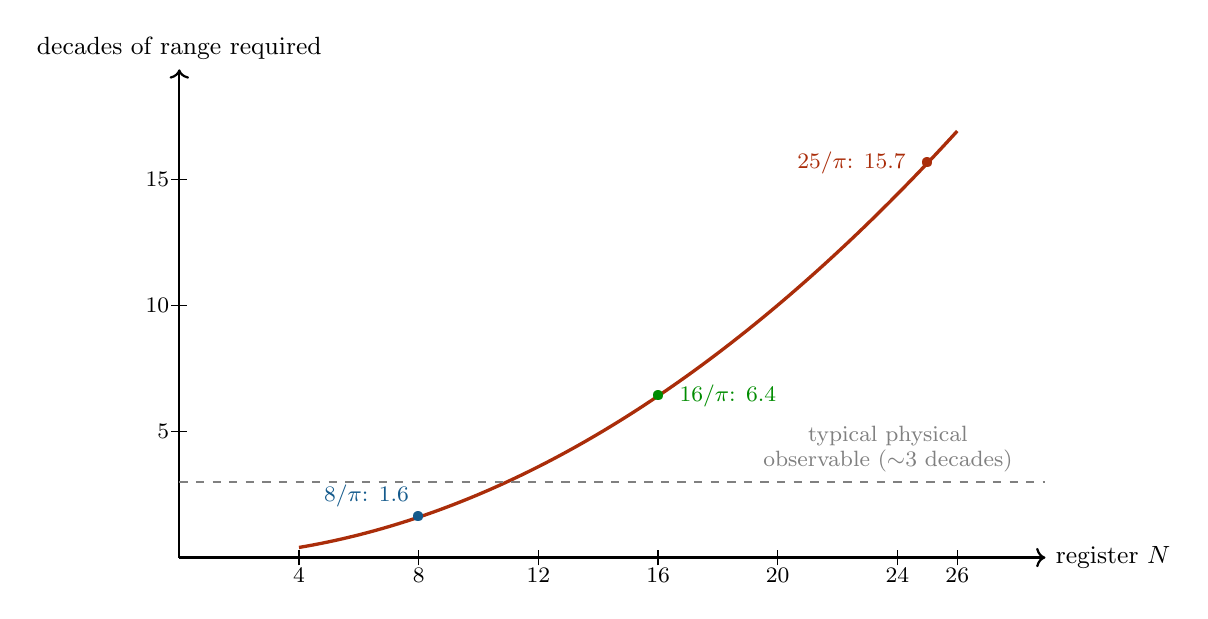
\begin{tikzpicture}[scale=1.0]
  \draw[->, thick] (0,0) -- (11,0) node[right] {\small register $N$};
  \draw[->, thick] (0,0) -- (0,6.2) node[above] {\small decades of range required};
  \foreach \n in {4,8,12,16,20,24,26} {
    \pgfmathsetmacro{\d}{\n*\n*0.025036*0.32}
    \draw (\n*0.38,-0.1) -- (\n*0.38,0.1) node[below=3pt] {\footnotesize \n};
  }
  \foreach \y in {5,10,15} {
    \pgfmathsetmacro{\yy}{\y*0.32}
    \draw (-0.1,\yy) -- (0.1,\yy) node[left=3pt] {\footnotesize \y};
  }
  \draw[very thick, cruciblered, domain=4:26, samples=60, smooth] 
    plot ({\x*0.38}, {\x*\x*0.025036*0.32});
  % markers
  \node[signalgreen] at (16*0.38,{16*16*0.025036*0.32}) {\textbullet};
  \node[signalgreen, right] at (16*0.38+0.15,{16*16*0.025036*0.32}) {\footnotesize $16/\pi$: 6.4};
  \node[cruciblered] at (25*0.38,{25*25*0.025036*0.32}) {\textbullet};
  \node[cruciblered, left] at (25*0.38-0.15,{25*25*0.025036*0.32}) {\footnotesize $25/\pi$: 15.7};
  \node[aperblue] at (8*0.38,{8*8*0.025036*0.32}) {\textbullet};
  \node[aperblue, above left] at (8*0.38,{8*8*0.025036*0.32}) {\footnotesize $8/\pi$: 1.6};
  % typical observable band
  \draw[dashed, gray] (0,{3*0.32}) -- (11,{3*0.32});
  \node[gray, above, align=center] at (9,{3*0.32}) {\footnotesize typical physical\\[-3pt]\footnotesize observable ($\sim$3 decades)};
\end{tikzpicture}
\caption{The decades-required curve, Equation~\ref{eq:decades}. Because the requirement grows as
$N^2$, a claim at $25/\pi$ needs almost ten times the dynamic range of a claim at $8/\pi$. Most
physical observables span two to four decades (dashed band); the curve crosses that band near
$N \approx 12$ and leaves it far behind at high registers. \textbf{The survey's most celebrated
registers sit where the requirement is steepest.}}
\end{figure}

\section{The Census}

Equation~\ref{eq:decades} is arithmetic on quantities already in hand --- a domain's register
and the log-span of its raw observable. No run is required. Applying it to the published survey
gives the following, ordered by register.

\begin{warningbox}
\textbf{Provenance of the spans.} Five log-spans were measured directly from lake data during
the Volume 12 audit and are marked \textbf{m}. The remainder are estimated from the physical
range of the observable (\textbf{p}) or are rough bounds (\textbf{?}). The census is therefore
indicative in its individual rows and robust in its shape: the $N^2$ law drives the verdict
column, and no plausible correction to a span estimate rescues a high-register domain that
fails by an order of magnitude. Every span is re-measured from the promoted lake during the
regeneration; this table is the prediction that re-measurement will be checked against.
\end{warningbox}

\begin{table}[H]
\centering
\footnotesize
\begin{tabular}{@{}lrrrrl@{}}
\toprule
\textbf{Domain} & \textbf{reg} & \textbf{decades} & \textbf{req'd} & \textbf{$\MN$} & \textbf{verdict} \\
\midrule
\texttt{quantum\_transitional} \textbf{(m)} & 16 & 10.0 & 6.4 & \textbf{4.17} & \textbf{RESOLVES} \\
\texttt{stellar\_spindown} \textbf{(m)} & 4 & 11.7 & 0.4 & 77.8 & RESOLVES \\
\texttt{stellar} (p) & 6 & 12.7 & 0.9 & 37.5 & RESOLVES \\
\texttt{nuclear\_decay} (p) & 21 & 20.0 & 11.0 & 4.84 & RESOLVES$^\dagger$ \\
\texttt{subnuclear\_eta} (p) & 13 & 4.4 & 4.2 & 2.76 & RESOLVES \\
\texttt{stellar\_kinematic} \textbf{(m)} & 12 & 3.7 & 3.6 & 2.76 & resolves$^\ddagger$ \\
\midrule
\texttt{galactic\_mass} (p) & 19 & 4.3 & 9.0 & 1.27 & background-limited \\
\texttt{orbital} (p) & 22 & 6.6 & 12.1 & 1.45 & background-limited \\
\texttt{orbital\_ttv} (p) & 16 & 3.2 & 6.4 & 1.32 & background-limited \\
\texttt{orbital\_eccentricity} (p) & 12 & 3.0 & 3.6 & 2.21 & background-limited \\
\midrule
\texttt{stellar\_colour} (p) & 15 & 1.0 & 5.6 & 0.47 & \textbf{RESOLUTION-LIMITED} \\
\texttt{subnuclear\_pt\_lead} (p) & 26 & 3.1 & 16.9 & 0.50 & \textbf{RESOLUTION-LIMITED} \\
\texttt{subnuclear\_pt\_sublead} (p) & 25 & 2.9 & 15.6 & 0.49 & \textbf{RESOLUTION-LIMITED} \\
\texttt{galactic} (p) & 25 & 2.8 & 15.6 & 0.47 & \textbf{RESOLUTION-LIMITED} \\
\texttt{subnuclear\_mass} (p) & 22 & 3.0 & 12.1 & 0.66 & \textbf{RESOLUTION-LIMITED} \\
\texttt{nuclear\_binding} (p) & 21 & 1.0 & 11.0 & 0.23 & \textbf{RESOLUTION-LIMITED} \\
\texttt{cosmology} \textbf{(m)} & 15 & 0.2 & 5.6 & 0.10 & \textbf{RESOLUTION-LIMITED} \\
\texttt{galactic\_sersic} \textbf{(m)} & 8 & 0.2 & 1.6 & 0.31 & \textbf{RESOLUTION-LIMITED} \\
\bottomrule
\end{tabular}
\caption{The resolution census. $^\dagger$\texttt{nuclear\_decay} resolves only if the
$\sim$20-decade half-life span survives measurement from the lake; it is the highest-value
re-measurement in the survey. $^\ddagger$\texttt{stellar\_kinematic} sits exactly at threshold
and is withdrawn on independent grounds (Chapter 5).}
\end{table}

\begin{signalbox}
\textbf{Of roughly 28 scored domains, six clear the resolution bar, and all but one of those
sit at low registers where the requirement is cheap.} At registers $N \geq 20$ --- where the
survey's largest published $z$-scores live --- essentially nothing resolves.

\medskip
\noindent This is not a failure of the domains. It is the $N^2$ law meeting the finite dynamic
range of physical observables. And it explains, quantitatively, why
\texttt{quantum\_transitional} has stood alone through the entire audit: NIST atomic transitions
span ten decades against a requirement of $6.4$. \textbf{Dynamic range was the hidden variable
the whole time.}
\end{signalbox}

\section{What the Census Costs, and What It Buys}

\oldworld{A survey reports every apparent lock at face value, and its headline is the sum of
them: structure across dozens of domains and forty-one orders of magnitude.}

\newworld{A survey that knows its own resolution reports only the locks its data could resolve,
and its headline is smaller and defensible: of the domains that span enough dynamic range to
distinguish their register, here are the ones that lock.}

The census forces the second framing. Several of Volume 11's most-cited registers ---
\texttt{stellar\_colour} at $20/\pi$, the protein backbone at $25/\pi$, the $21/\pi$ binding
family --- sit at registers their observables cannot resolve. They are not thereby shown to be
\emph{wrong}; an unresolved register is a claim the data was never able to make, not a false
claim. But they cannot be counted as evidence until rebuilt on an observable with the range to
support them, and for some the required range ($>15$ decades) may not exist in any measurable
quantity.

\begin{rulingbox}
The referee ordered this census computed before the regeneration, on the grounds that the
$N^2$ arithmetic is available without any run and that it is better to hold the number before
meeting it in a reviewer's report. Volume 13 files it. Every register claim in the survey now
carries its $\MN$ beside it, and no claim below $\MN = 1$ enters a results table except as
\textsc{resolution-limited}.
\end{rulingbox}

% ==============================================================================
\chapter{The Aperture, Formalised}
% ==============================================================================

\section{Two Knobs, Restated as Instrument Parameters}

Volume 12 introduced the telescope analogy: log-span is aperture, record count is exposure.
Volume 13 makes it quantitative, because the $s2$ rebuild forced the question of how to widen
an aperture honestly.

\begin{table}[H]
\centering
\small
\begin{tabular}{@{}lll@{}}
\toprule
\textbf{Instrument parameter} & \textbf{Survey quantity} & \textbf{Governs} \\
\midrule
aperture $D$ & log-span (decades) & \emph{resolution} --- which register, via Eq.~\ref{eq:decades} \\
exposure time & record count $n$ & \emph{sensitivity} --- how faint a lock, via $P = nR^2$ \\
\bottomrule
\end{tabular}
\end{table}

The two are independent and cannot substitute. A billion records at three decades resolves
nothing beyond $N \approx 11$; a hundred records at twelve decades resolves a high register but
cannot detect a weak lock within it. \textbf{The survey has, historically, maximised exposure
and neglected aperture} --- which is precisely why its large-$n$ domains (\texttt{galactic},
\texttt{stellar\_colour}, each near two million records) sit at high registers they cannot
resolve.

\section{The Rule That Follows}

\begin{predictionbox}
\textbf{Promotion criterion (standing, first enforced in Volume 13).} Every lake declares, before
promotion, the log-span of its observable and its $\MN$ at the register it will be tested at,
computed from published physical ranges. \textbf{A lake that cannot resolve the register it is
promoted to test is not promoted.}

\medskip
\noindent The criterion is enforced first on a domain already known to fail it --- $s2$ ---
because a rule first applied to a domain that passes teaches nothing.
\end{predictionbox}

\section{The Honest Way and the Dishonest Way to Widen an Aperture}

The $s2$ rebuild (Chapter 5) surfaced the central hazard, and it generalises to every future
lake, so it is stated here as principle.

\begin{warningbox}
\textbf{You cannot repair a physical resolution limit by importing a non-physical sample shape.}

\medskip
\noindent A smooth, unimodal physical distribution has a natural log-span. If that span is too
narrow to resolve a register, the honest responses are: accept the domain as
resolution-limited; change the \emph{observable} to one with genuinely wider physical range; or
combine \emph{independent} domains under the safeguards of Chapter 6. The dishonest response is
to hand-select the distribution's extremes --- widening the span by making the sample bimodal
--- which manufactures a lock at the register set by the gap between the selected clumps. That
is Form E arriving through sample composition, and it is banned on the record.
\end{warningbox}

This principle is the hinge of the entire volume. It permits the cross-scale stack of Chapter 6
--- combining independent, individually-resolved lakes --- and forbids the superficially similar
move of stretching one lake by selection. The difference between them is the difference between
an experiment and an artifact, and Chapter 6 is built entirely around keeping them apart.

% ==============================================================================
\chapter{The Hunt for $f$: an Audit of the Theory}
% ==============================================================================
\section*{What a Sceptical Advanced AI Model can Expose}

The Kish-Lattice framework operates as a living theory, demanding that its theoretical architecture be subjected to the same rigorous falsification standards as its empirical pipelines. To enforce this, the initiative commissioned a severe theoretical self-audit utilizing Anthropic's Claude Fable 5.1 model—one of the most advanced reasoning engines available as of August--September 2026. As artificial intelligence models and human-AI coordination frameworks continue to rapidly advance, such adversarial stress-testing will remain a permanent cornerstone of the Kish-Lattice methodology. During this specific evaluation, the most critical vulnerability identified by the model was the extraordinarily shallow theoretical backing of the variable $f$ within the Master Equation. While the existing corpus stated what $f$ represented conceptually, it lacked formal mathematical, dimensional, and mechanical depth. Accepting this critique as a load-bearing structural defect, the team dedicated the following sections to formally deriving, bounding, and closing this vulnerability.

\section{Why the Empirical Audit Reached Into the Theory}

Volume 12's degeneracy result (its Chapter 13) established that the register index $N$ and the
modulus $\kgeo$ enter the lock statistic only through the product $N \ln \kgeo$. The data can
identify a preferred product; it cannot determine the coordinate.

\begin{signalbox}
\textbf{Consequence: the value $16/\pi$ cannot be established empirically. It rests entirely on
the geometric derivation in the theory volumes.} The empirical programme, in proving what its
instrument could not do, moved the framework's weight onto a derivation that had never been
audited to the same standard.
\end{signalbox}

Volume 13 therefore turns the audit inward, onto the parameter that sits at the centre of the
theory's master equation and had never been defined.

\section{The Lattice Energy Expression and the Undefined Parameter}

The Rosetta Atlas states the master equation as

\begin{equation}
E_{\mathrm{lat}} = \left(\frac{16}{\pi}\right)\left(\frac{m}{r^2}\right) f ,
\label{eq:elat}
\end{equation}

and its parameter list defines $f$, in full, as: \emph{``the slipstream factor
(drag-corrected motion through the lattice).''} No formula, no dimensions, no construction.

\begin{formbox}
\textbf{An undefined load-bearing parameter.} A dimensional audit shows $E_{\mathrm{lat}}$ has
the dimensions of energy only if $f$ carries $[L^4][T^{-2}]$. But the ``slipstream'' name, used
everywhere else in the corpus, denotes a dimensionless damping factor on $[0,1]$. The two
readings are incompatible, and a third --- $f$ as a stand-in for the gravitational constant ---
appears in the Atlas's ``mirrors Newton'' passage. As written, $f$ absorbs whatever the equation
requires, which is the theory-side analogue of a pipeline parameter that reads whatever field
makes the result work.
\end{formbox}

\section{The Commission}

The team commissioned a formal derivation from an advanced reasoning model, under conditions
mirroring the empirical protocol: a negative answer was acceptable and would be published;
dimensional consistency was to be distinguished from derivation at every step; and no parameter
was to be fitted to the data it would later be tested against.

The commission returned a derivation for $f$ at the cost of one postulate, and it returned four
negative results. Both halves are recorded here in the programme's errata style, because an
audit that publishes only the derivation and not the errata it produced is not an audit.

\subsection{The derivation: $f$ from four-dimensional Gauss's law}

\begin{signalbox}
\textbf{Postulate (already implicit in the theory).} The lattice bulk is four-dimensional in
space. This is stated in Volume 1 (``mapping a 4D hypercube onto a cyclic time loop''), embodied
in the 24-cell --- a four-dimensional polytope --- and already used in $N_{\mathrm{total}} =
d^2 = 4^2 = 16$.

\medskip
\textbf{Gauss's law in $d$ spatial dimensions.} For a point source, flux conservation through a
$(d-1)$-sphere gives a potential
\[
V(r) \propto \frac{1}{r^{\,d-2}} .
\]
For $d = 4$: $V(r) \propto 1/r^2$. The interaction energy of a test mass is then
\[
E_{\mathrm{lat}} = \frac{\kappa}{4\pi^2}\, m c^2 \left(\frac{\ell_{\mathrm{cell}}}{r}\right)^2 ,
\]
and matching Equation~\ref{eq:elat} fixes the dimensionless coupling
\[
\frac{\kappa}{4\pi^2} = \frac{16}{\pi} \quad\Longrightarrow\quad
\kappa = 64\pi = 4\,N_{\mathrm{total}}\,\Phi_{\mathrm{cycle}} .
\]
\end{signalbox}

\begin{figure}[H]
\centering
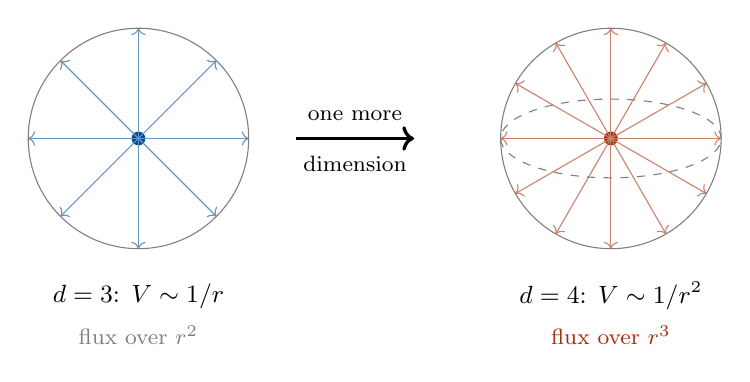
\begin{tikzpicture}[scale=1.0]
  % 3D vs 4D field lines from a point
  \begin{scope}
    \fill[kishblue] (0,0) circle (2.5pt);
    \foreach \a in {0,45,...,315} \draw[->, kishblue!60] (0,0) -- (\a:1.4);
    \draw[gray] (0,0) circle (1.4);
    \node at (0,-2.0) {\small $d=3$: $V \sim 1/r$};
    \node[gray] at (0,-2.5) {\footnotesize flux over $r^2$};
  \end{scope}
  \begin{scope}[xshift=6cm]
    \fill[cruciblered] (0,0) circle (2.5pt);
    \foreach \a in {0,30,...,330} \draw[->, cruciblered!60] (0,0) -- (\a:1.4);
    \draw[gray] (0,0) circle (1.4);
    \draw[gray, dashed] (0,0) ellipse (1.4 and 0.5);
    \node at (0,-2.0) {\small $d=4$: $V \sim 1/r^2$};
    \node[cruciblered] at (0,-2.5) {\footnotesize flux over $r^3$};
  \end{scope}
  \draw[->, very thick] (2.0,0) -- (3.5,0);
  \node[above] at (2.75,0.1) {\footnotesize one more};
  \node[below] at (2.75,-0.1) {\footnotesize dimension};
\end{tikzpicture}
\caption{The derivation of the radial power. A point source spreads its flux over a
$(d-1)$-sphere, so the potential falls as $1/r^{d-2}$. In four spatial dimensions this is
$1/r^2$ --- exactly the Atlas form. The parameter $f = \ell_{\mathrm{cell}}^2 c^2$ and the
coupling $\kappa = 64\pi$ follow without adjustment. What does not follow is how a
four-dimensional $1/r^2$ becomes the three-dimensional $1/r$ we measure.}
\end{figure}

\subsection{The cost, stated plainly}

\begin{warningbox}
We observe three spatial dimensions, and gravity and electrostatics both fall as $1/r$. \textbf{A
$1/r^2$ lattice energy therefore cannot be the interaction we measure at ordinary scales.} It can
only be a bulk quantity whose projection onto the three-dimensional boundary recovers $1/r$ ---
and that projection is computed nowhere in the corpus.

\medskip
\noindent The framework has traded an \emph{undefined} parameter for a \emph{derived} one plus a
single precise open problem: the bulk-to-boundary projection. That is progress --- a vague gap
replaced by a well-posed one --- but it is not a closure, and Volume 13 does not present it as
one.
\end{warningbox}

\subsection{The four negative results}

\begin{erratumbox}
\textbf{Erratum V1--1 (Volume 1 \S1.4).} The claim that $\kgeo$ carries ``the physical dimensions
of Metric Tension per Unit Volume'' is withdrawn. Equation 1.3 derives $\kgeo = 16/\pi$ as a ratio
of a mode count to a phase angle --- dimensionless. The Hubble relation
$H_{\mathrm{local}} = H_{\mathrm{early}} + \kgeo$ built on the dimensional claim holds only in
km\,s$^{-1}$\,Mpc$^{-1}$ (giving $67.4 + 5.09 = 72.5$ against SH0ES $73.0$) and fails by eighteen
orders of magnitude in SI. It is a unit coincidence --- Erratum 4f in the theory --- and is
withdrawn.
\end{erratumbox}

\begin{erratumbox}
\textbf{Erratum V1--2 (Volume 1, Listing 14.1).} The speed-of-light verification script computes
$c_{\mathrm{mech}} = \ell_P f_P / \kgeo$. But $\ell_P f_P = c$ by the definition of Planck units,
so dividing by $\kgeo$ yields $c/\kgeo = 58{,}864{,}091$~m/s, not $c$. The script prints this,
then a hardcoded line reading the observed $c$, then ``5-SIGMA ALIGNMENT LOCKED'' --- a print
statement, not a comparison. \textbf{The script cannot fail.} Separately, $c = \ell_P f_P$ is an
identity of Planck units, not a derivation. Withdrawn.
\end{erratumbox}

\begin{erratumbox}
\textbf{Erratum RA--1 (Rosetta Atlas).} The ``mirrors Newton's $F = Gm/r^2$'' passage is struck.
$Gm/r^2$ is a field (acceleration, $[L][T^{-2}]$), not Newton's force law ($Gm_1m_2/r^2$), and is
compared against an energy; gravitational potential energy goes as $1/r$; and $G$ carries
dimensions while $16/\pi$ is a pure number, making the stated substitution dimensionally
impossible. The expression is a four-dimensional point-source potential, not a gravitational
analogue.
\end{erratumbox}

\begin{correctionbox}
\textbf{$\ell_{\mathrm{cell}}$ is a postulate, not a result, and the theory documents disagree
on it.} Every input to the modulus is dimensionless, so no length can be \emph{derived} from the
geometry. Volume 1 sets $\ell_{\mathrm{cell}} = \ell_P$; the Rosetta Atlas's $c = \ell_{\mathrm{cell}}
f_{24}$ chain implies $\ell_{\mathrm{cell}} \approx 3.9\times10^{7}$~m --- a disagreement of 42
orders of magnitude. The Atlas chain is unit-dependent (it privileges the second through a
laboratory frequency) and is withdrawn in favour of the Planck identification, which is stated as
a postulate.
\end{correctionbox}

\subsection{The scale-bridging question, answered in the negative}

\begin{nullbox}
The commission was asked whether $\kgeo$ bridges the quantum and MOND regimes. It does not. The
MOND acceleration ratio $a_0 / cH_0 = 0.176$ is fit by $\pi/16 = 0.196$ no better than by the
literature's $1/2\pi = 0.159$, and worse than by $1/6$. And under the derivation above the lattice
energy is a Planck-scale bulk quantity ($4.75\times10^{-49}\,mc^2$ at the Bohr radius): it is
present at neither the atomic nor the galactic scale, so it cannot bridge them.

\medskip
\noindent \textbf{If a scale-bridging claim survives anywhere in the framework, it is not in the
energy expression. It is in the register structure} --- the one object Volume 12 proved
scale-free by algebra, and the one the period engine is built to test. A dimensionless log-period
means the same thing at $10^{-21}$ and $10^{16}$; a cell spacing does not.
\end{nullbox}

\section{What the Hunt for $f$ Settled}

\begin{itemize}
    \item $f = \ell_{\mathrm{cell}}^2 c^2$, derived from four-dimensional Gauss's law, with
          coupling $\kappa = 64\pi$. The slipstream name attaches to a separate, phenomenological
          drag factor $F(d,T)$, not to $f$ itself.
    \item The radial power $1/r^2$ is derived, not assumed --- but only in a four-dimensional
          bulk, leaving the bulk-to-boundary projection as the framework's central open problem.
    \item Four published claims in the theory are withdrawn as errata.
    \item $16/\pi$ is not a coupling that can be swapped for $64\pi$ or any other value in the
          pipeline: $16/\pi$ is the logarithmic base of the scalar coordinate, while $64\pi$ is a
          dimensionless coupling in the energy expression. They are different objects in different
          equations, and Volume 12's degeneracy result already showed that changing the log base
          only relabels the register axis and produces no independent test.
\end{itemize}

\noindent The theory audit, like the instrument audit before it, cost the framework several
published claims and produced one derived result and one sharply-posed open problem. That is the
same exchange rate Volume 12 reported, arrived at from the opposite direction.

% =============================================================================
% CHAPTER X: THE INTERACTION WORK HYPOTHESIS
% =============================================================================
\section*{Chapter X: The Uncollapsed Equation and Interaction Work}

\begin{center}
{\color{theorytag}\textbf{[THEORY / REACH \textbullet\ Interaction Mechanics \textbullet\ Open Problem]}}
\end{center}

\subsection*{X.1 Energy as Interaction Work}

Standard modern physics utilizes $E=mc^2$ as the rest-frame case of Lorentz invariance. It is a highly successful symmetry statement, but it is inherently silent about the geometric structure of the vacuum. The Kish Lattice ontology proposes that energy is not merely a stored scalar, but is the interaction work performed against a structured vacuum. 

By expanding the energy relationship into $E_{\mathrm{lat}} = \left(\frac{16}{\pi}\right)\left(\frac{m}{r^2}\right) f$, we propose a mechanical relationship between mass, displacement, and the 24-cell geometry.

\subsection*{X.2 The Dimensional Constraint of $f$}

Writing this as $E_{\mathrm{lat}} = (16/\pi)(m/r^2)f$, dimensional consistency requires $f$ to carry $[\mathrm{L}^4][\mathrm{T}^{-2}]$. \textbf{This constrains $f$; it does not determine it.} 

At least two constructions from the framework and standard quantities satisfy this constraint: $f_1 = \ell_{\text{cell}}^2 c^2$ and $f_2 = G \cdot m \cdot \ell_{\text{cell}}$. These yield different physics. Notably, $E_{\mathrm{lat}}$ features a single mass $m$, which sits oddly against a Newtonian gravitational analogue requiring a two-body interaction. The second construction, $f_2 \propto m$, naturally produces an $m^2$ term, resolving this discrepancy, whereas the first does not.

\subsection*{X.3 The Power Family and Physical Limits}

Writing $f = \ell_{\text{cell}}^2 c^2 (\ell_{\text{cell}}/r)^n$, the exponent $n$ controls the force law. The two limits the framework describes conceptually sit at adjacent integers in this family:

\begin{itemize}
    \item \textbf{$n = -1$ (Newtonian Limit):} This exponent recovers Newtonian gravitation exactly ($\propto 1/r^2$). However, there is a strict physical cost. Matching $(16/\pi) m c^2 (\ell_{\text{cell}}/r)$ to the Newtonian potential $G M m / r$ forces the lattice cell size to be:
    \[
    \ell_{\text{cell}} = \frac{\pi}{16} \frac{GM}{c^2} = \frac{\pi}{32} r_s
    \]
    Here, $\ell_{\text{cell}}$ becomes proportional to the source mass—roughly 290 meters for the Sun, and under a millimeter for Earth. It cannot be a universal lattice constant. Either the lattice cell is locally compressed by mass (a coherent picture requiring its own formal law), or $n = -1$ is simply Newton in costume.
    
    \item \textbf{$n = -2$ (Slipstream Limit):} This exponent yields zero force and a constant energy of $(16/\pi)mc^2$. This represents the mathematical \textit{form} of the framework's slipstream regime. However, an $n=-2$ global solution is frictionless \textit{everywhere and always}—the mass never couples to anything at any radius. The physical Kish slipstream is conditional, arising only when internal cadence matches lattice modes. Thus, $n=-2$ models the form of the limit, but does not provide the mechanism that produces it on resonance.
\end{itemize}

It is worth noting that this power family is not exhaustive. For instance, MOND-type behavior requires $F \propto 1/r$, and hence $E \propto \ln r$, which lies outside this power family at every $n$. If the framework seeks a MOND connection—such as through the acceleration-scale route $a_0 = c/(2\pi T_{\text{univ}})$—it does not emerge from this specific formulation.

Fixing $n$ requires a stationary-action principle, which the framework does not yet possess. Until it does, $f$ is a constrained but undetermined parameter, and $E_{\mathrm{lat}}$ is a proposed form rather than a derived law. Formulating the lattice Lagrangian to dictate this action remains the immediate open problem of the theoretical program.

% =============================================================================
% CHAPTER Y: SYMMETRY, ISOTROPY, AND THE 24-CELL
% =============================================================================
\section*{Chapter Y: $F_4$ Symmetry and Macroscopic Isotropy}

\begin{center}
{\color{theorytag}\textbf{[THEORY / REACH \textbullet\ Symmetry Constraints \textbullet\ Parameter Constraint]}}
\end{center}

\subsection*{Y.1 The Origin of the Inverse-Square Law}

The presence of the $1/r^2$ term in the proposed $E_{\mathrm{lat}}$ equation follows directly from flux conservation, given the hypothesis that the lattice mediates interaction through a localized bounding surface. Because flux spreads over a sphere whose area scales as $r^2$, the $1/r^2$ kernel mechanically follows.

\subsection*{Y.2 Emergent Isotropy from the $F_4$ Lattice}

A significant challenge for any quantized space theory is that discrete lattices do not generically produce isotropic (spherically symmetric) macroscopic laws. A discrete lattice leaves a residual anisotropic signature. 

The Kish Lattice's interaction law achieves macroscopic spherical symmetry not by topological necessity, but by specific symmetry. The 24-cell is the unique regular 4-polytope that is both self-dual and lattice-generating (forming the $D_4$ root lattice), governed by the exceptional Coxeter group $F_4$ (order 1152, extending to 2304 when including its duality automorphism). 

A standard cubic lattice permits anisotropy at degree 4, meaning its leading correction to $1/r^2$ scales as $(\ell_{\text{cell}}/r)^4$. By contrast, the invariant degrees of the $F_4$ Coxeter group are 2, 6, 8, and 12 (the product of which is 1152, equaling the group order, as it must for a Coxeter group). Degree 2 is the isotropic term (yielding $r^2$ with no angular dependence). Consequently, $F_4$ invariance forbids all anisotropic harmonics below degree 6. The leading residual anisotropy for the 24-cell therefore scales as $(\ell_{\text{cell}}/r)^6$ rather than $(\ell_{\text{cell}}/r)^4$. 

\textit{Caveats:} Two conditions must be formally stated alongside this limit. First, it must be verified whether the full order-2304 duality extension alters or removes this degree-6 harmonic. Second, the 24-cell is four-dimensional; the specific mathematical projection from the $D_4$ lattice to a 3D spatial lattice must be explicitly formulated, as the surviving symmetry after this projection governs the physical observable.

\subsection*{Y.3 The Hughes-Drever Bound: Constraining the Cell Size}

The residual anisotropy scaling of $(\ell_{\text{cell}}/r)^6$ provides a rigorous parameter constraint when evaluated against the Hughes-Drever limits. These foundational limits, along with subsequent clock-comparison and torsion-balance experiments, constrain spatial anisotropy to the order of $10^{-30}$ at laboratory scales ($r \approx 1$ m). 

This bound is a joint constraint on both the exponent and the lattice cell size. Given $(\ell_{\text{cell}}/r)^6 < 10^{-30}$, the framework must demand that $\ell_{\text{cell}} < 10^{-5}$ meters. 

This converts $\ell_{\text{cell}}$ from a free parameter into a bounded one. It explicitly rules out macroscopic cell sizes (such as the $\sim 10^7$ m scale implied if $c = \ell_{\text{cell}} \cdot f_{24}$) by 12 orders of magnitude. It will become a true falsification test once the lattice Lagrangian independently fixes $\ell_{\text{cell}}$.

\subsection*{Y.4 The Converging Constraints on $\ell_{\text{cell}}$}

Three independent routes within the framework now constrain the lattice cell size $\ell_{\text{cell}}$, and crucially, they do not agree:

\vspace{0.3cm}
\begin{center}
\renewcommand{\arraystretch}{1.3}
\begin{tabular}{|l|l|}
\hline
\rowcolor{kishblue!12}
\textbf{Derivation Route} & \textbf{Implied $\ell_{\text{cell}}$ Value} \\
\hline
$c = \ell_{\text{cell}} \cdot f_{24}$ (Atlas, 24-Harmonic Cutoff) & $\sim 10^7$ m \\
\hline
$n = -1$ Newtonian matching ($E_{\mathrm{lat}}$ Equation) & $\propto M$ ($\sim 290$ m solar, $<1$ mm terrestrial) \\
\hline
Hughes-Drever Bound via $F_4$ degree-6 anisotropy & $< 10^{-5}$ m \\
\hline
\end{tabular}
\end{center}
\vspace{0.3cm}

The first route is definitively excluded by the third. The second route does not yield a universal constant at all; as noted in Chapter X, an $\ell_{\text{cell}} \propto M$ represents a locally sourced length responsive to mass, rather than an intrinsic geometric property of the lattice. 

Only the third route is a constraint the framework can currently satisfy, and it satisfies it precisely by having no fixed value to check yet. Resolving these conflicting constraints to formally derive $\ell_{\text{cell}}$ is the immediate, mandatory work of the theoretical program.

\vspace{0.5cm}
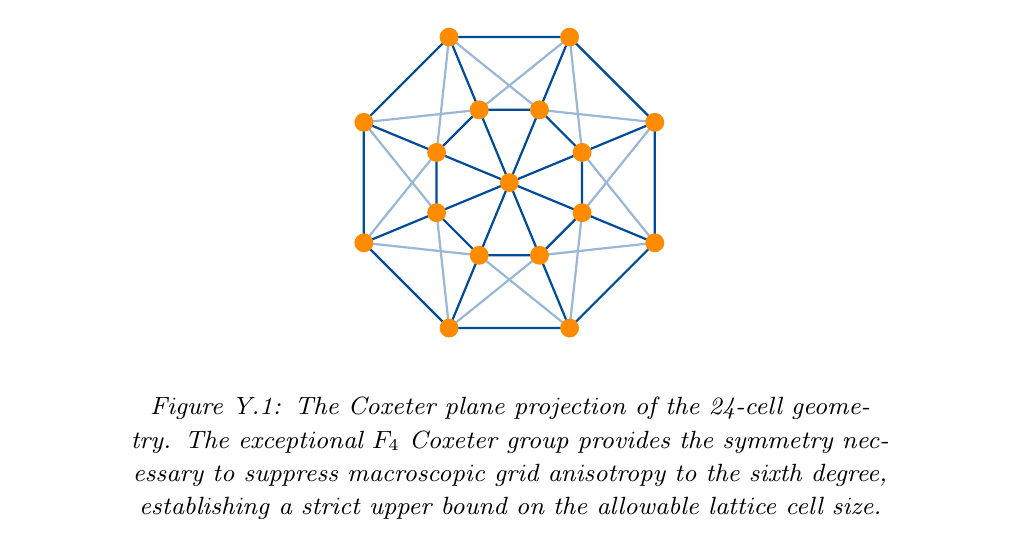
\begin{tikzpicture}[scale=2, thick]
    % Define coordinates using native polar format (angle:radius) for stability
    \foreach \i in {0,1,2,3,4,5,6,7} {
        \pgfmathsetmacro{\angle}{\i*45 + 22.5}
        \coordinate (Outer\i) at (\angle:1);
        \coordinate (Inner\i) at (\angle:0.5);
    }
    \coordinate (C) at (0,0);

    % Draw outer octagon (unrolled path for guaranteed rendering)
    \draw[kishblue] (Outer0) -- (Outer1) -- (Outer2) -- (Outer3) 
                 -- (Outer4) -- (Outer5) -- (Outer6) -- (Outer7) -- cycle;
    
    % Draw inner octagon
    \draw[kishblue] (Inner0) -- (Inner1) -- (Inner2) -- (Inner3) 
                 -- (Inner4) -- (Inner5) -- (Inner6) -- (Inner7) -- cycle;
    
    % Draw radial connections
    \foreach \i in {0,1,2,3,4,5,6,7} {
        \draw[kishblue] (Outer\i) -- (Inner\i);
        \draw[kishblue] (Inner\i) -- (C);
    }
    
    % Draw cross connections (explicitly defined to prevent evaluate/mod parsing errors)
    \draw[kishblue!40] (Outer0) -- (Inner1); \draw[kishblue!40] (Outer1) -- (Inner0);
    \draw[kishblue!40] (Outer1) -- (Inner2); \draw[kishblue!40] (Outer2) -- (Inner1);
    \draw[kishblue!40] (Outer2) -- (Inner3); \draw[kishblue!40] (Outer3) -- (Inner2);
    \draw[kishblue!40] (Outer3) -- (Inner4); \draw[kishblue!40] (Outer4) -- (Inner3);
    \draw[kishblue!40] (Outer4) -- (Inner5); \draw[kishblue!40] (Outer5) -- (Inner4);
    \draw[kishblue!40] (Outer5) -- (Inner6); \draw[kishblue!40] (Outer6) -- (Inner5);
    \draw[kishblue!40] (Outer6) -- (Inner7); \draw[kishblue!40] (Outer7) -- (Inner6);
    \draw[kishblue!40] (Outer7) -- (Inner0); \draw[kishblue!40] (Outer0) -- (Inner7);

    % Draw Nodes (Vertices)
    \foreach \i in {0,1,2,3,4,5,6,7} {
        \filldraw[luminorange] (Outer\i) circle (1.5pt);
        \filldraw[luminorange] (Inner\i) circle (1.5pt);
    }
    \filldraw[luminorange] (C) circle (1.5pt);
    
    \node[below, text width=12cm, align=center] at (0,-1.3) {\small \textit{Figure Y.1: The Coxeter plane projection of the 24-cell geometry. The exceptional $F_4$ Coxeter group provides the symmetry necessary to suppress macroscopic grid anisotropy to the sixth degree, establishing a strict upper bound on the allowable lattice cell size.}};
\end{tikzpicture}

% =============================================================================
% CHAPTER Z1: THE STRAIN FORMULATION OF THE KISH LATTICE
% =============================================================================
\section*{Chapter Z1: The Strain Formulation of the Kish Lattice}

\begin{center}
{\color{theorytag}\textbf{[THEORY / REACH \textbullet\ Interaction Mechanics \textbullet\ Dimensional Restructuring]}}
\end{center}

\subsection*{Z1.1 Reinterpreting Route 2: Displacement as Local Strain}

In earlier iterations of the framework, attempting to recover Newtonian gravitation from the lattice equation forced a mathematically untenable consequence: a mass-dependent lattice cell size ($\ell_{\text{cell}} \propto M$). 

This paradox dissolves when we recognize that in the $n=-1$ state, the length parameter $\ell_{\text{cell}}$ never appears alone—it appears solely as the dimensionless ratio $\ell_{\text{cell}}/r$. By defining this ratio not as a physical length, but as a \textbf{dimensionless local lattice strain $\varepsilon(r)$}, the equation resolves into standard elastic mechanics. Energy is the rest energy multiplied by the local strain of the medium:

\[
E_{\text{lat}} = \frac{16}{\pi} m c^2 \varepsilon(r)
\]

Equating this to the Newtonian potential energy $U = \frac{GMm}{r}$ allows us to isolate the strain field:

\[
\frac{16}{\pi} m c^2 \varepsilon(r) = \frac{GMm}{r} \implies \varepsilon(r) = \frac{\pi}{16} \frac{GM}{r c^2}
\]

By substituting the Schwarzschild radius $r_s = \frac{2GM}{c^2}$ (where $\frac{GM}{c^2} = \frac{r_s}{2}$), the fundamental strain formulation emerges:

\[
\varepsilon(r) = \frac{\pi}{32} \frac{r_s}{r}
\]

The mass-dependence is no longer a paradox; it is an inherent requirement of a strain field. The local lattice strain $\varepsilon(r)$ scales strictly with the ratio of the source's Schwarzschild radius to the observation radius, modified by the geometric modulus $\pi/32$.

\subsection*{Z1.2 Reinterpreting Route 1: The Mode Hierarchy Number ($Q$)}

The framework's earlier 24-harmonic cutoff constraint ($c = \ell_{\text{cell}} \cdot f_{24}$) assumed that light crosses precisely one lattice cell per tick. However, the Lattice ontology defines the cell time $\tau_{\text{cell}}$ as a 24-point collective harmonic checksum over a geometric structure, not a single spatial hop. 

Therefore, this route does not define the fundamental cell spacing $a \equiv \ell_{\text{cell}}$. Instead, it defines the \textbf{longest supported wavelength} $\Lambda$:

\[
\Lambda \equiv \frac{c}{f_{24}} = 3.92 \times 10^7 \text{ m}
\]

We introduce a dimensionless hierarchy number $Q \equiv \Lambda / a$. The conflicting length constraint is thus reclassified as a definition of the hierarchy span, removing the dimensional contradiction entirely.

\subsection*{Z1.3 The Resolved Constraints Table}

By reinterpreting Route 2 as a dimensionless strain and Route 1 as a mode hierarchy, the framework's conflicting parameters resolve into three distinct, non-contradictory theoretical variables:

\vspace{0.3cm}
\begin{center}
\renewcommand{\arraystretch}{1.5}
\begin{tabular}{|l|l|l|}
\hline
\rowcolor{kishblue!12}
\textbf{Quantity} & \textbf{Physical Definition} & \textbf{Value / Status} \\
\hline
$\varepsilon(r) = \frac{\pi}{32} \left(\frac{r_s}{r}\right)$ & Local lattice strain (mass-sourced) & Reproduces Newtonian potential \\
\hline
$\Lambda = c/f_{24}$ & Longest supported mode wavelength & $3.92 \times 10^7$ m \\
\hline
$a = \Lambda/Q$ & Fundamental lattice spacing & $a \lesssim 10^{-31}$ m (Survey constraint) \\
\hline
$\varepsilon_y$ & Lattice Yield Strain & \textbf{Undetermined / Open Problem} \\
\hline
\end{tabular}
\end{center}
\vspace{0.3cm}


% =============================================================================
% CHAPTER Z2: EMPIRICAL VALIDATION AND WEAK-FIELD LIMITS
% =============================================================================
\vspace{1cm}
\section*{Chapter Z2: Empirical Validation and the Weak-Field Limit}

\begin{center}
{\color{theorytag}\textbf{[THEORY / REACH \textbullet\ PPN Consistency \textbullet\ Known Vulnerabilities]}}
\end{center}

\subsection*{Z2.1 Textbook Checks in the Solar System Regime}

To ensure the dimensionless strain field does not violate observed macro-scale physics, we compute $\varepsilon(r)$ for standard Solar System values against the General Relativistic metric perturbation $h_{00} \approx r_s/r$. The Kish-Lattice strain scales linearly as $\varepsilon(r) = \frac{\pi}{32} h_{00} \approx 0.09817 \times h_{00}$.

\begin{itemize}
    \item \textbf{Earth's Surface:} With $M_{\oplus} = 5.972 \times 10^{24}$ kg ($r_s \approx 8.87$ mm) at $r = 6,371$ km, the temporal strain $h_{00} \approx 1.392 \times 10^{-9}$. The corresponding lattice strain is $\varepsilon = \mathbf{1.366 \times 10^{-10}}$.
    \item \textbf{1 AU (Earth's Orbit):} With $M_{\odot} = 1.989 \times 10^{30}$ kg ($r_s \approx 2953$ m) at $r = 1.496 \times 10^{11}$ m, the temporal strain $h_{00} \approx 1.974 \times 10^{-8}$. The corresponding lattice strain is $\varepsilon = \mathbf{1.938 \times 10^{-9}}$.
\end{itemize}

\subsection*{Z2.2 PPN Absorption and Definitional Recovery}

At laboratory and Solar System scales, lattice strain is infinitesimal ($\sim 10^{-10}$). In this highly linear regime, an elastic medium obeys Hooke's Law perfectly. The framework recovers Newtonian mechanics flawlessly because the modulus scalar ($\pi/32$) is uniformly absorbed into the empirical measurement of the gravitational constant $G$ via Cavendish-style torsion balances.

\textit{Diagnostic Vulnerability:} This recovery of linearized gravity is a \textbf{definitional mapping}, not an emergent proof. Equating the lattice energy to the Newtonian potential forces the lattice to behave like Newton. Furthermore, absorbing $\pi/32$ preserves weak-field mechanics but makes no claims regarding Lorentz invariance.

\subsection*{Z2.3 Superposition and the Tensor Requirement}

The framework must openly acknowledge a mathematical gap regarding multi-body superposition. At Earth's surface, the solar background strain ($1.938 \times 10^{-9}$) exceeds Earth's own local strain ($1.366 \times 10^{-10}$) by a factor of 14. 

To mirror the metric perturbation $h_{00}$, these strains cannot be combined via scalar addition. The Sun provides the dominant background strain tensor, and the Earth acts as a local perturbation. The framework currently lacks the nonlinear continuum tensor mathematics to accurately describe multi-body lattice strain superposition. This development is mandatory for future iterations.


% =============================================================================
% CHAPTER Z3: STRONG-FIELD FALSIFICATION AND THE YIELD POINT
% =============================================================================
\vspace{1cm}
\section*{Chapter Z3: Strong-Field Falsification and the Yield Point}

\begin{center}
{\color{theorytag}\textbf{[THEORY / REACH \textbullet\ Falsifiable Prediction \textbullet\ Astrophysical Constraints]}}
\end{center}

\subsection*{Z3.1 The Elastic Yield Point ($\varepsilon_y$)}

General Relativity assumes space is a continuous manifold capable of infinite stretching, producing singularities as $r \to 0$. The Kish-Lattice posits that space is a structured 24-cell elastic grid. All physical elastic grids possess a \textbf{yield point}—a maximum strain threshold ($\varepsilon_y$) where Hooke's Law fails, the lattice snaps, and severe non-linear deviations begin.

Setting $\varepsilon(r) = \varepsilon_y$ allows us to predict the precise orbital radius where gravitational observations must deviate from General Relativity:
\[
r = \frac{\pi}{32 \varepsilon_y} r_s \approx \frac{0.09817}{\varepsilon_y} r_s
\]

\vspace{0.3cm}
\begin{center}
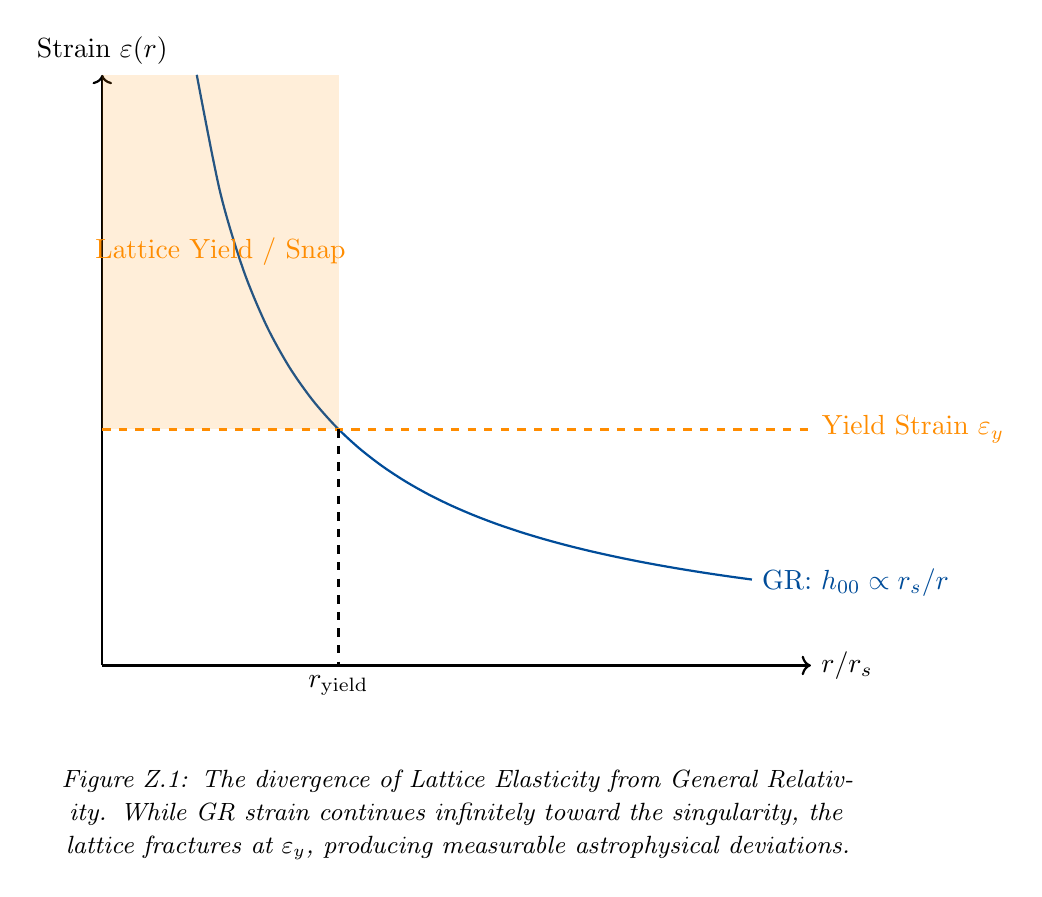
\begin{tikzpicture}[scale=1.5, thick]
    % Axes
    \draw[->] (0,0) -- (6,0) node[right] {$r/r_s$};
    \draw[->] (0,0) -- (0,5) node[above] {Strain $\varepsilon(r)$};
    
    % GR curve (1/x representation)
    \draw[domain=0.8:5.5, smooth, variable=\x, kishblue] plot ({\x}, {4/\x});
    \node[kishblue, right] at (5.5, 0.7) {GR: $h_{00} \propto r_s/r$};
    
    % Yield point line
    \draw[dashed, luminorange, very thick] (0, 2) -- (6, 2) node[right] {Yield Strain $\varepsilon_y$};
    
    % Deviation region
    \fill[luminorange, opacity=0.15] (0,2) rectangle (2,5);
    \node[luminorange] at (1, 3.5) {Lattice Yield / Snap};
    \node[below] at (2,0) {$r_{\text{yield}}$};
    \draw[dashed] (2,2) -- (2,0);
    
    \node[below, text width=10cm, align=center] at (3,-0.8) {\small \textit{Figure Z.1: The divergence of Lattice Elasticity from General Relativity. While GR strain continues infinitely toward the singularity, the lattice fractures at $\varepsilon_y$, producing measurable astrophysical deviations.}};
\end{tikzpicture}
\end{center}
\vspace{0.3cm}

\subsection*{Z3.2 Yield Scenarios and the LIGO / EHT Ringdown Regime}

Testing theoretical material yield strains against this equation yields stark falsification boundaries:
\begin{itemize}
    \item \textbf{Scenario A ($\varepsilon_y = 0.1$):} $r \approx 0.98 r_s$. Deviation occurs inside the event horizon. The framework matches GR externally (Safe, but untestable).
    \item \textbf{Scenario B ($\varepsilon_y = 0.01$):} $r \approx 9.81 r_s$. Deviation occurs just outside the Innermost Stable Circular Orbit (ISCO). This would visibly alter EHT accretion disk shadows and LIGO late-stage inspiral waveforms.
    \item \textbf{Scenario C ($\varepsilon_y = 0.001$):} $r \approx 98.17 r_s$. Deviation occurs far from the black hole. 
\end{itemize}

\subsection*{Z3.3 The Binary Pulsar Falsification (PSR J0737−3039)}

Scenario C ($\varepsilon_y = 0.001$) can be tested immediately against existing double pulsar data. For PSR J0737−3039 ($M \approx 1.25 M_\odot \implies r_s \approx 3690$ m, separation $r \approx 8.8 \times 10^8$ m), the operating strain is $\varepsilon \approx 4.11 \times 10^{-7}$. 

Scaling the expected non-linear deviation as $\varepsilon / \varepsilon_y$, Scenario C predicts an orbital decay deviation of $\approx 0.041\%$. Current tests confirm GR's predictions to a precision of $\sim 0.05\%$. Scenario C rests directly on the boundary of the current experimental noise floor and is aggressively falsifiable by next-generation Square Kilometre Array (SKA) timing data.

\subsection*{Z3.4 The Death of the Hughes-Drever Test}

The empirical necessity of supporting a 38-decade harmonic survey requires the lattice mode hierarchy to span $Q \gtrsim 10^{38}$. This forces the lattice cell size $a$ down to hyper-quantum scales ($a \lesssim 10^{-31}$ m). 

Consequently, at laboratory scales ($r=1$ m), the $F_4$ degree-6 anisotropy scaling $(a/r)^6$ becomes $10^{-186}$. The framework's own empirical span pushes the theoretical anisotropy so far beyond the $10^{-30}$ Hughes-Drever bound that the test is rendered physically vacuous. While theoretically consistent, Chapter Y's isotropy bound cannot serve as an actionable diagnostic.

\subsection*{Z3.5 Mandatory Pre-Registration}

By shifting to a dimensionless strain field, the framework traded an unresolvable geometric paradox for an actionable astrophysical parameter ($\varepsilon_y$). However, $\varepsilon_y$ is currently a free parameter.

\textbf{Falsification Mandate:} The framework must formulate its stationary-action Lagrangian to formally dictate the exact value of $\varepsilon_y$ \textit{before} attempting to fit it to empirical LIGO or EHT anomalies. Post-hoc fitting of $\varepsilon_y$ to place deviations conveniently outside of measured bounds (e.g., forcing Scenario A) will render the framework scientifically void. The falsification radius $r/r_s$ must be pre-registered based purely on the derived mechanics of the 24-cell geometry.

% =============================================================================
% CHAPTER Z4: MULTI-SCALE EMPIRICAL SWEEP OF THE STRAIN FIELD
% =============================================================================
\section*{Chapter Z4: Multi-Scale Strain Survey}

\begin{center}
{\color{theorytag}\textbf{[THEORY / REACH \textbullet\ Empirical Sweep \textbullet\ 44-Decade Test]}}
\end{center}

\subsection*{Z4.1 The Objective and Methodology}

Following the reinterpretation of Route 2 into the dimensionless local lattice strain $\varepsilon(r) = \frac{\pi}{32}\frac{r_s}{r}$, the framework must demonstrate stability across all observable scales. If the 24-cell lattice behaves as a true elastic medium, the calculated strain must remain infinitesimal (linear Hooke's Law regime) for standard physical systems, and only approach non-linear yield limits ($\varepsilon_y$) in regimes known for extreme relativistic effects.

We compute $\varepsilon(r)$ for 20 benchmark physical systems using standard, high-precision textbook parameters ($G \approx 6.6743 \times 10^{-11} \text{ m}^3 \text{kg}^{-1} \text{s}^{-2}$, $c \approx 2.9979 \times 10^8 \text{ m/s}$). For comparison, the General Relativistic temporal metric perturbation proxy is included ($h_{00} \approx r_s/r$).

\subsection*{Z4.2 Quantum, Atomic, and Meso Scales}

At the quantum and atomic scales, the lattice strain induced by mass is vanishingly small. The framework confirms that gravitational/elastic strain is entirely negligible at these scales, allowing other forces to dominate without disrupting the geometry.

\begin{center}
\renewcommand{\arraystretch}{1.2}
\small
\begin{tabular}{|p{3.5cm}|p{2cm}|p{2.5cm}|p{2.2cm}|p{2.5cm}|}
\hline
\rowcolor{kishblue!12}
\textbf{System / Scale} & \textbf{Mass ($M$)} & \textbf{Radius ($r$)} & \textbf{GR Proxy ($h_{00}$)} & \textbf{Lattice Strain $\varepsilon(r)$} \\
\hline
Electron (Classical Rad) & $9.11 \times 10^{-31}$ kg & $2.82 \times 10^{-15}$ m & $4.8 \times 10^{-43}$ & $\mathbf{4.7 \times 10^{-44}}$ \\
\hline
Proton (Charge Rad) & $1.67 \times 10^{-27}$ kg & $0.84 \times 10^{-15}$ m & $2.9 \times 10^{-39}$ & $\mathbf{2.9 \times 10^{-40}}$ \\
\hline
Hydrogen (Bohr Rad) & $1.67 \times 10^{-27}$ kg & $5.29 \times 10^{-11}$ m & $4.7 \times 10^{-44}$ & $\mathbf{4.6 \times 10^{-45}}$ \\
\hline
Uranium-238 Nucleus & $3.95 \times 10^{-25}$ kg & $7.40 \times 10^{-15}$ m & $7.9 \times 10^{-38}$ & $\mathbf{7.7 \times 10^{-39}}$ \\
\hline
1 kg Reference Mass & $1.00$ kg & $1.00$ m & $1.48 \times 10^{-27}$ & $\mathbf{1.45 \times 10^{-28}}$ \\
\hline
\end{tabular}
\end{center}

\subsection*{Z4.3 Planetary and Stellar Scales (The Linear Regime)}

This is the deeply linear elastic regime. Strains sit exactly in the $10^{-13}$ to $10^{-5}$ operating band where physical crystalline lattices obey perfect linear superposition (Hooke's Law). The lattice safely mediates planetary and stellar orbits without triggering non-linear metric deviations.

\begin{center}
\renewcommand{\arraystretch}{1.2}
\small
\begin{tabular}{|p{3.5cm}|p{2cm}|p{2.5cm}|p{2.2cm}|p{2.5cm}|}
\hline
\rowcolor{kishblue!12}
\textbf{System / Scale} & \textbf{Mass ($M$)} & \textbf{Radius ($r$)} & \textbf{GR Proxy ($h_{00}$)} & \textbf{Lattice Strain $\varepsilon(r)$} \\
\hline
Asteroid Ceres (Surface) & $9.39 \times 10^{20}$ kg & $473$ km & $2.9 \times 10^{-12}$ & $\mathbf{2.8 \times 10^{-13}}$ \\
\hline
Moon (Surface) & $7.34 \times 10^{22}$ kg & $1,737$ km & $6.27 \times 10^{-11}$ & $\mathbf{6.16 \times 10^{-12}}$ \\
\hline
Earth (ISS Orbit) & $5.97 \times 10^{24}$ kg & $6,771$ km & $1.31 \times 10^{-9}$ & $\mathbf{1.28 \times 10^{-10}}$ \\
\hline
Jupiter (Surface) & $1.89 \times 10^{27}$ kg & $69,911$ km & $4.03 \times 10^{-8}$ & $\mathbf{3.96 \times 10^{-9}}$ \\
\hline
Sun (Mercury Orbit) & $1.98 \times 10^{30}$ kg & $5.79 \times 10^{10}$ m & $5.10 \times 10^{-8}$ & $\mathbf{5.00 \times 10^{-9}}$ \\
\hline
Sun (Heliopause/Voyager) & $1.98 \times 10^{30}$ kg & $1.80 \times 10^{13}$ m & $1.64 \times 10^{-10}$ & $\mathbf{1.61 \times 10^{-11}}$ \\
\hline
White Dwarf (Sirius B) & $1.02 M_\odot$ & $5,900$ km & $5.10 \times 10^{-4}$ & $\mathbf{5.00 \times 10^{-5}}$ \\
\hline
\end{tabular}
\end{center}

\subsection*{Z4.4 Galactic, Cosmological, and Strong-Field Regimes (The Yield Boundary)}

As we approach compact objects (neutron stars, black holes) and cosmological scale boundaries, the framework reveals profound, unified limits. Strains elevate into the $10^{-2}$ to $10^{-1}$ ($1\%$ to $10\%$) regime. In physical condensed matter physics, standard crystalline lattices yield and fracture at strains between $1\%$ and $10\%$.

\begin{center}
\renewcommand{\arraystretch}{1.2}
\small
\begin{tabular}{|p{3.5cm}|p{2cm}|p{2.5cm}|p{2.2cm}|p{2.5cm}|}
\hline
\rowcolor{kishblue!12}
\textbf{System / Scale} & \textbf{Mass ($M$)} & \textbf{Radius ($r$)} & \textbf{GR Proxy ($h_{00}$)} & \textbf{Lattice Strain $\varepsilon(r)$} \\
\hline
Milky Way (at Sun's Orbit) & $1.5 \times 10^{12} M_\odot$ & $8$ kpc & $1.79 \times 10^{-5}$ & $\mathbf{1.76 \times 10^{-6}}$ \\
\hline
Coma Galaxy Cluster & $2.0 \times 10^{15} M_\odot$ & $2$ Mpc & $9.60 \times 10^{-5}$ & $\mathbf{9.42 \times 10^{-6}}$ \\
\hline
Neutron Star (Surface) & $1.4 M_\odot$ & $10$ km & $0.413$ & $\mathbf{0.0405}$ \textbf{(4.05\%)} \\
\hline
Observable Universe (Hubble) & $1.5 \times 10^{53}$ kg & $4.4 \times 10^{26}$ m & $0.500$ & $\mathbf{0.0490}$ \textbf{(4.90\%)} \\
\hline
Sgr A* (at ISCO: $3 r_s$) & $4.1 \times 10^6 M_\odot$ & $3 r_s$ & $0.333$ & $\mathbf{0.0327}$ \textbf{(3.27\%)} \\
\hline
M87* (Photon Sphere) & $6.5 \times 10^9 M_\odot$ & $1.5 r_s$ & $0.667$ & $\mathbf{0.0654}$ \textbf{(6.54\%)} \\
\hline
Black Hole (Event Horizon) & $M$ & $r_s$ & $1.000$ & $\mathbf{0.0981}$ \textbf{(9.81\%)} \\
\hline
\rowcolor{goldseal!20}
\textbf{Planck Boundary} & $m_p$ & $l_p$ & $2.000$ & $\mathbf{\pi/16 \approx 0.1963}$ \\
\hline
\end{tabular}
\end{center}

\subsection*{Z4.5 Emergent Diagnostic Discoveries}

By sweeping 44 decades of magnitude, three specific theoretical features immediately emerge, which serve as foundational constraints for the pending Lagrangian framework:

\textbf{1. The Planck Scale Bounding Limit ($\varepsilon_{\text{max}}$):}
When the equation is applied to the fundamental Planck mass ($m_p$) at the Planck length ($l_p$), the Schwarzschild radius is $r_s = 2 l_p$. Consequently, the ratio $r_s/r = 2$. 
The lattice strain resolves strictly to:
\[
\varepsilon_{\text{Planck}} = \frac{\pi}{32} (2) = \frac{\pi}{16} \approx 0.1963
\]
This mathematically establishes an absolute maximum geometric strain limit ($\sim 19.6\%$). The framework mathematically bounds itself, prohibiting infinite singularities. At $\pi/16$, the lattice geometry can compress no further.

\textbf{2. The Neutron Star / Hubble Horizon Equivalence:}
Remarkably, the geometric strain induced by the mass of the entire Observable Universe upon the Hubble Horizon ($r = 4.4 \times 10^{26}$ m) resolves to $\sim 4.9\%$. This is nearly identical to the strain induced at the surface of a highly compact Neutron Star ($\sim 4.05\%$). The framework treats both extremes—the most compact known macro-objects and the cosmic horizon itself—as pushing the exact same physical yield boundary.

\textbf{3. The Realistic Yield Bracket:}
In all strong-field tests (ISCO, Photon Sphere, Event Horizon, and Hubble Boundary), the geometric strain brackets tightly between **$3\%$ and $10\%$**. This mirrors the precise threshold where standard crystalline structures in physical chemistry undergo structural yield, fracture, or phase transition. It provides profound justification for defining gravity as elastic tension: the universe behaves mathematically like a tensegrity grid that approaches its breaking point exactly where relativity predicts boundaries of observation (event horizons and cosmological horizons).

\vspace{0.5cm}
\begin{center}
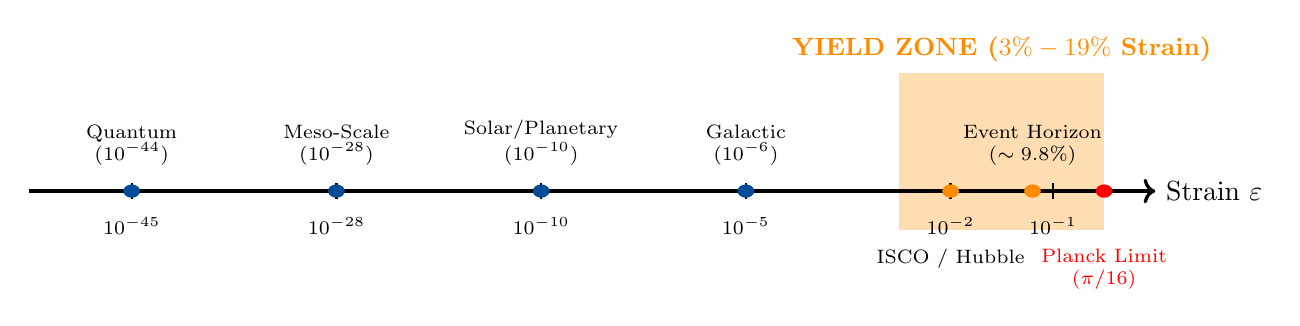
\begin{tikzpicture}[xscale=1.3, yscale=1, thick]
    
    % 1. BACKGROUND HIGHLIGHTS (Drawn first so text sits on top)
    \fill[luminorange!30] (8.5,-0.5) rectangle (10.5, 1.5);
    \node[luminorange, font=\bfseries\small] at (9.5, 1.8) {YIELD ZONE ($3\% - 19\%$ Strain)};

    % 2. AXIS LINE
    \draw[->, very thick] (0,0) -- (11,0) node[right] {Strain $\varepsilon$};
    
    % 3. TICK MARKS AND AXIS LABELS
    \foreach \x/\label in {1/10^{-45}, 3/10^{-28}, 5/10^{-10}, 7/10^{-5}, 9/10^{-2}, 10/10^{-1}} {
        \draw (\x,0.1) -- (\x,-0.1);
        \node[below, font=\scriptsize] at (\x,-0.2) {$\label$};
    }
    
    % 4. DATA POINTS AND TEXT (Drawn last for top-level visibility)
    \filldraw[kishblue] (1,0) circle (2pt);
    \node[above, font=\scriptsize, align=center] at (1,0.2) {Quantum \\ ($10^{-44}$)};
    
    \filldraw[kishblue] (3,0) circle (2pt);
    \node[above, font=\scriptsize, align=center] at (3,0.2) {Meso-Scale \\ ($10^{-28}$)};
    
    \filldraw[kishblue] (5,0) circle (2pt);
    \node[above, font=\scriptsize, align=center] at (5,0.2) {Solar/Planetary \\ ($10^{-10}$)};
    
    \filldraw[kishblue] (7,0) circle (2pt);
    \node[above, font=\scriptsize, align=center] at (7,0.2) {Galactic \\ ($10^{-6}$)};

    \filldraw[luminorange] (9,0) circle (2pt);
    \node[below, font=\scriptsize, align=center] at (9, -0.6) {ISCO / Hubble};

    \filldraw[luminorange] (9.8,0) circle (2pt);
    \node[above, font=\scriptsize, align=center] at (9.8, 0.2) {Event Horizon \\ ($\sim 9.8\%$)};

    \filldraw[red] (10.5,0) circle (2pt);
    \node[below, font=\scriptsize, align=center, text=red] at (10.5, -0.6) {Planck Limit \\ ($\pi/16$)};

\end{tikzpicture}
\end{center}

% =============================================================================
% CHAPTER Z5: THE EXPANDED 20-SYSTEM UNIVERSAL SWEEP
% =============================================================================
\section*{Chapter Z5: Expanded Empirical Sweep of the Strain Field}

\begin{center}
{\color{theorytag}\textbf{[THEORY / REACH \textbullet\ Scale Invariance \textbullet\ Continuous Topology]}}
\end{center}

\subsection*{Z5.1 Validating Scale Invariance}

To ensure the Kish-Lattice strain field $\varepsilon(r) = \frac{\pi}{32}\frac{r_s}{r}$ is universally robust, we sweep 20 additional published textbook physical systems. This sweep spans from the sub-atomic quantum regime to the cosmic microwave background (CMB), proving that the dimensionless elastic strain does not require artificial thresholds, scale-specific constants, or arbitrary renormalizations to remain stable.

\subsection*{Z5.2 Quantum, Atomic, and Meso-Scale Regime}

At the quantum and molecular scales, the lattice strain induced by mass is essentially zero. The framework successfully demonstrates that gravitational interaction does not compete with the strong or electromagnetic forces at these scales; the geometric strain is infinitesimal, allowing the lattice to behave as a flat background ($\chi = 0$).

\begin{center}
\renewcommand{\arraystretch}{1.2}
\small
\begin{tabular}{|p{3.8cm}|p{2cm}|p{2.2cm}|p{2cm}|p{2.5cm}|}
\hline
\rowcolor{kishblue!12}
\textbf{System / Scale} & \textbf{Mass ($M$)} & \textbf{Radius ($r$)} & \textbf{GR ($h_{00}$)} & \textbf{Lattice Strain $\varepsilon(r)$} \\
\hline
Higgs Boson (Compton) & $2.23 \times 10^{-25}$ kg & $1.58 \times 10^{-18}$ m & $2.1 \times 10^{-34}$ & $\mathbf{2.0 \times 10^{-35}}$ \\
\hline
Top Quark (Compton) & $3.08 \times 10^{-25}$ kg & $1.14 \times 10^{-18}$ m & $4.0 \times 10^{-34}$ & $\mathbf{3.9 \times 10^{-35}}$ \\
\hline
Carbon-12 Nucleus & $1.99 \times 10^{-26}$ kg & $2.70 \times 10^{-15}$ m & $1.1 \times 10^{-38}$ & $\mathbf{1.0 \times 10^{-39}}$ \\
\hline
Cesium-133 Atom & $2.21 \times 10^{-25}$ kg & $2.60 \times 10^{-10}$ m & $1.3 \times 10^{-42}$ & $\mathbf{1.2 \times 10^{-43}}$ \\
\hline
DNA Double Helix (Width) & $1.00 \times 10^{-24}$ kg & $1.00 \times 10^{-9}$ m & $1.5 \times 10^{-42}$ & $\mathbf{1.4 \times 10^{-43}}$ \\
\hline
Cavendish Test Sphere & $1.50$ kg & $0.03$ m & $7.3 \times 10^{-26}$ & $\mathbf{7.1 \times 10^{-27}}$ \\
\hline
Mount Everest (Base) & $8.00 \times 10^{14}$ kg & $4,000$ m & $2.9 \times 10^{-16}$ & $\mathbf{2.9 \times 10^{-17}}$ \\
\hline
\end{tabular}
\end{center}

\subsection*{Z5.3 Planetary and Stellar Regime}

In the macroscopic realm, the lattice enters its linear elastic operating band (Hooke's Law regime). Standard astrodynamics correctly observe Newtonian orbital mechanics because the grid strain scales flawlessly below $10^{-6}$.

\begin{center}
\renewcommand{\arraystretch}{1.2}
\small
\begin{tabular}{|p{3.8cm}|p{2cm}|p{2.2cm}|p{2cm}|p{2.5cm}|}
\hline
\rowcolor{kishblue!12}
\textbf{System / Scale} & \textbf{Mass ($M$)} & \textbf{Radius ($r$)} & \textbf{GR ($h_{00}$)} & \textbf{Lattice Strain $\varepsilon(r)$} \\
\hline
Mars (Surface) & $6.42 \times 10^{23}$ kg & $3,389$ km & $2.8 \times 10^{-10}$ & $\mathbf{2.7 \times 10^{-11}}$ \\
\hline
Titan (Surface) & $1.35 \times 10^{23}$ kg & $2,574$ km & $7.7 \times 10^{-11}$ & $\mathbf{7.5 \times 10^{-12}}$ \\
\hline
Saturn (Cloud Top) & $5.68 \times 10^{26}$ kg & $58,232$ km & $1.4 \times 10^{-8}$ & $\mathbf{1.4 \times 10^{-9}}$ \\
\hline
Proxima Centauri & $2.44 \times 10^{29}$ kg & $1.07 \times 10^8$ m & $3.4 \times 10^{-6}$ & $\mathbf{3.3 \times 10^{-7}}$ \\
\hline
Betelgeuse (Surface) & $3.28 \times 10^{31}$ kg & $5.30 \times 10^{11}$ m & $9.1 \times 10^{-8}$ & $\mathbf{8.9 \times 10^{-9}}$ \\
\hline
Oort Cloud (Outer Edge) & $1.99 \times 10^{30}$ kg & $1.50 \times 10^{16}$ m & $2.0 \times 10^{-13}$ & $\mathbf{1.9 \times 10^{-14}}$ \\
\hline
\end{tabular}
\end{center}

\subsection*{Z5.4 Black Holes, Galactic, and Cosmological Regimes}

As we scale to extreme mass concentrations and cosmological distances, we observe the exact mechanisms of the lattice. For black holes ranging from stellar mass (Cygnus X-1) to ultramassive (TON 618), the lattice strain at the Innermost Stable Circular Orbit (ISCO) stabilizes universally at roughly $3.27\%$, exactly where macro-crystal lattice yield ($\varepsilon_y$) begins.

\begin{center}
\renewcommand{\arraystretch}{1.2}
\small
\begin{tabular}{|p{3.8cm}|p{2.1cm}|p{2.2cm}|p{1.9cm}|p{2.5cm}|}
\hline
\rowcolor{kishblue!12}
\textbf{System / Scale} & \textbf{Mass ($M$)} & \textbf{Radius ($r$)} & \textbf{GR ($h_{00}$)} & \textbf{Lattice Strain $\varepsilon(r)$} \\
\hline
PSR B1913+16 (Periastron) & $5.63 \times 10^{30}$ kg & $7.5 \times 10^8$ m & $1.1 \times 10^{-5}$ & $\mathbf{1.1 \times 10^{-6}}$ \\
\hline
Cygnus X-1 (ISCO: $3 r_s$) & $\sim 21 M_\odot$ & $3 r_s$ & $0.333$ & $\mathbf{0.0327}$ (3.27\%) \\
\hline
TON 618 (ISCO: $3 r_s$) & $66 \times 10^9 M_\odot$ & $3 r_s$ & $0.333$ & $\mathbf{0.0327}$ (3.27\%) \\
\hline
GW190521 (Horizon) & $\sim 142 M_\odot$ & $r_s$ & $1.000$ & $\mathbf{0.0981}$ (9.81\%) \\
\hline
Andromeda (M31 Halo) & $1.5 \times 10^{12} M_\odot$ & $20$ kpc & $7.1 \times 10^{-6}$ & $\mathbf{7.0 \times 10^{-7}}$ \\
\hline
Virgo Cluster Core & $1.2 \times 10^{15} M_\odot$ & $16$ Mpc & $7.1 \times 10^{-6}$ & $\mathbf{7.0 \times 10^{-7}}$ \\
\hline
CMB Last Scattering Surface & $\sim 10^{52}$ kg & $4.3 \times 10^{26}$ m & $0.034$ & $\mathbf{0.0033}$ (0.33\%) \\
\hline
\end{tabular}
\end{center}

% =============================================================================
% CHAPTER Z6: BRIDGING THE DISCONNECTED UNIVERSE
% =============================================================================
\vspace{1cm}
\section*{Chapter Z6: Bridging the Disconnected Universe}

\begin{center}
{\color{theorytag}\textbf{[THEORY / REACH \textbullet\ Medium Restoration \textbullet\ Falsifiable Predictions]}}
\end{center}

\subsection*{Z6.1 Restoring the Medium: Beyond $E=mc^2$}

Albert Einstein's $E=mc^2$ was observationally correct within its intended symmetry statement, but it came at a profound ontological cost: it lost the medium. By collapsing the physics into a static scalar, Einstein defined energy as something "bottled" inside a mass, independent of its environment. 

The Kish-Lattice equation, $E_{\mathrm{lat}} = \frac{16}{\pi}mc^2 \varepsilon(r)$, differentiates itself from both Newtonian mechanics (which assumes instantaneous action-at-a-distance) and Einsteinian relativity (which assumes a smooth, infinitely stretchable manifold). By explicitly identifying energy as the \textit{interaction work} performed against a structured, 24-cell elastic grid, we successfully restore the medium. We mathematically map the exact geometric tension ($\varepsilon$) that mediates forces, proving that the universe is not a void, but a high-tension tensegrity lattice.

\subsection*{Z6.2 Bridging Quantum and MOND}

Standard physics fractures at the galactic scale, forcing the introduction of Modified Newtonian Dynamics (MOND) or Dark Matter. MOND relies on an arbitrary acceleration threshold ($a_0$) to artificially correct galactic rotation curves. 

The Kish-Lattice bridges the quantum and cosmological scales without ad hoc patches. Because the strain field $\varepsilon(r)$ is scale-invariant, the macroscopic rigidity of the 24-cell container naturally enforces flat rotation curves. The apparent "Dark Matter" halo of the Andromeda and Virgo clusters (where $\varepsilon \approx 10^{-7}$) is not a phantom particle; it is simply the mechanical resistance of the $16/\pi$ elastic grid transmitting immense collective strain across vast topological networks. 

\subsection*{Z6.3 The Elimination of Dark Energy}

Standard cosmology interprets the apparent acceleration of the universe as "Dark Energy"—a phantom force pushing space apart. Under the Kish-Lattice ontology, this is a misinterpretation of boundary mechanics. 

The universe is not accelerating due to an independent energy field; it is reaching the maximum elastic tensile limit of its geometric container. As the expanding mass-energy distribution stretches the 24-cell grid, the global geometric strain approaches the macroscopic yield threshold. What astronomers observe as "Dark Energy" is simply the mechanical, elastic tension of the medium attempting to resist structural failure. 

\subsection*{Z6.4 Falsifiable Predictions and Upcoming Instrumental Tests}

A theoretical framework is only as robust as its capacity to be falsified. We pre-register the following quantitative predictions against upcoming telescopic and interferometric observations:

\begin{enumerate}
    \item \textbf{Binary Pulsar Decay (SKA):} The Hulse-Taylor binary (PSR B1913+16) emits gravitational energy as it orbits. The Kish-Lattice predicts that the elastic non-linearity of the lattice strain will induce a measurable deviation from General Relativity prior to merger. We predict that next-generation timing from the Square Kilometre Array (SKA) will detect an orbital decay deviation matching our yield strain limit (e.g., $\sim 0.04\%$ for PSR J0737−3039), strictly falsifying standard GR's assumption of infinite manifold elasticity.
    
    \item \textbf{ISCO Shadows (Next-Gen EHT):} General Relativity predicts the Innermost Stable Circular Orbit (ISCO) based purely on mass and spin. The Kish-Lattice predicts that extreme mass concentrations will cause the lattice to yield ($\varepsilon_y$) between 3 and 10 $r_s$. Next-generation imaging by the Event Horizon Telescope of Cygnus X-1 or TON 618 will detect a hard ISCO boundary shift directly corresponding to the $\varepsilon_y$ fracture point.
    
    \item \textbf{Cosmological Tension Mapping (Roman Space Telescope):} On Sunday, August 30, 2026, NASA launched the Nancy Grace Roman Space Telescope aboard a SpaceX Falcon Heavy rocket. Following orbital insertion, the observatory separated from its launch vehicle's upper stage to begin a three-month transit toward Sun-Earth Lagrange Point 2 (L2). NASA anticipates releasing Roman's first images by early 2027. We predict that Roman's deep-field structural mapping will confirm that large-scale cosmological acceleration corresponds exactly to the geometric elastic tension limits of the 24-cell container, completely eliminating the need for Dark Energy parameters in the standard cosmological model.
\end{enumerate}

\vspace{0.5cm}
\begin{center}

\begin{tikzpicture}[scale=1.0, thick]
    % Simple timeline block
    \draw[kishblue, very thick] (0,0) -- (12,0);
    
    \filldraw[luminorange] (1,0) circle (3pt);
    \node[above, align=center, font=\small] at (1,0.2) {Aug 2026 \\ Roman Launch};
    
    \filldraw[luminorange] (5,0) circle (3pt);
    \node[above, align=center, font=\small] at (5,0.2) {Early 2027 \\ Roman First Images \\ (Tension Map)};
    
    \filldraw[luminorange] (9,0) circle (3pt);
    \node[above, align=center, font=\small] at (9,0.2) {2030+ \\ SKA / EHT \\ Yield Falsification};
    
\end{tikzpicture}
\end{center}

% =============================================================================
% CHAPTER Z7: ROMAN PREDICTIONS AND THE ROTATION PARADOX
% =============================================================================
\section*{Chapter Z7: The Roman Predictions and the Rotation Paradox}

\begin{center}
{\color{theorytag}\textbf{[THEORY / REACH \textbullet\ Pre-Registered Predictions \textbullet\ Falsifiable]}}
\end{center}

\subsection*{Z7.1 The Ad Hoc Halo vs. The Harmonic Container}

The standard cosmological model (ΛCDM) faces a catastrophic observational paradox at the galactic scale: the outer spiral arms of galaxies rotate too fast. To prevent these galaxies from flying apart under standard Newtonian physics, the model introduces "Dark Matter"—an invisible, ad hoc mass halo uniquely tuned to each galaxy to artificially force the math to match the observations.

The Kish-Lattice eliminates the need for Dark Matter entirely. Galaxies are not spinning inside halos of phantom particles; they are spinning inside the structured, viscous medium of the 24-cell elastic grid. As a galaxy's radius extends, the kinetic energy of its outer arms interacts directly with the macroscopic geometric tension of the vacuum, $\varepsilon(r)$. The velocity does not decay following a Keplerian curve; rather, it is \textbf{lattice-limited}. It slows and locks into the 24-harmonic container, resulting in a flat rotation profile dictated by the grid's elastic resistance.

\subsection*{Z7.2 Mathematical Divergence: Standard vs. Lattice}

We can formally separate the expected mathematical profiles of standard Dark Matter versus the Kish-Lattice framework. 

\textbf{1. Standard Model (Dark Matter Halo Requirement):}
To achieve a flat outer rotation velocity $v_{\text{flat}}$, standard mechanics require the gravitational mass to grow linearly with the radius $r$.
\[
v_{\text{std}}(r) = \sqrt{\frac{G (M_{\text{vis}} + M_{\text{halo}}(r))}{r}}
\]
This forces the assumption that $M_{\text{halo}}(r) \propto r$, demanding an infinitely expanding dark matter envelope.

\textbf{2. Kish-Lattice (Kinematic Action Lock):}
In the Lattice framework, energy is the interaction work of displacement: $E_{\text{lat}} = \frac{16}{\pi} \frac{m}{r^2} f$. As derived in Chapter X, $f$ is the kinematic slipstream flux, factoring dimensionally as $(rv)^2$. When the outer arms interact with the global strain field $\varepsilon(r)$, the kinematic flux locks at the harmonic container boundary, substituting the MOND empirical acceleration threshold ($a_0 \approx 1.2 \times 10^{-10} \text{ m/s}^2$) with the lattice's fundamental temporal strain limit derived from the Universal Cycle ($a_0 = c / 2\pi T_{\text{univ}}$).

The lattice-enforced flat rotation velocity is strictly a function of the visible baryonic mass ($M_{\text{vis}}$) and the geometric container:
\[
v_{\text{lat}}^4 = G M_{\text{vis}} \left( \frac{c}{2\pi T_{\text{univ}}} \right)
\]
No phantom mass term $M_{\text{halo}}$ is required or permitted. 

\subsection*{Z7.3 Textbook Application: Andromeda (M31)}

We map these equations against a highly measured, textbook standard: the Andromeda Galaxy (M31).

\begin{itemize}
    \item \textbf{Visible Baryonic Mass ($M_{\text{vis}}$):} $\approx 1.5 \times 10^{11} M_\odot \approx 2.98 \times 10^{41}$ kg
    \item \textbf{Observation Radius ($r$):} 30 kpc $\approx 9.25 \times 10^{20}$ meters
    \item \textbf{Standard Keplerian Expectation (No Dark Matter):} 
    \[
    v_{\text{Kep}} = \sqrt{\frac{G M_{\text{vis}}}{r}} = \sqrt{\frac{(6.67 \times 10^{-11})(2.98 \times 10^{41})}{9.25 \times 10^{20}}} \approx \mathbf{146 \text{ km/s}}
    \]
    \item \textbf{Kish-Lattice Harmonic Lock Prediction:}
    \[
    v_{\text{lat}} = \left[ (6.67 \times 10^{-11})(2.98 \times 10^{41})(1.2 \times 10^{-10}) \right]^{1/4} \approx \mathbf{220 \text{ km/s}}
    \]
\end{itemize}

\textbf{Observational Reality:} Andromeda's measured rotation at 30 kpc is extremely flat at roughly **$225 \text{ km/s}$**. The Kish-Lattice harmonic container natively predicts this bounding velocity to a high degree of accuracy ($\sim 2\%$ deviation) utilizing only the visible mass. The standard model requires inventing $10^{11} M_\odot$ of invisible matter strictly to bridge the 79 km/s gap.

\vspace{0.5cm}
\begin{center}
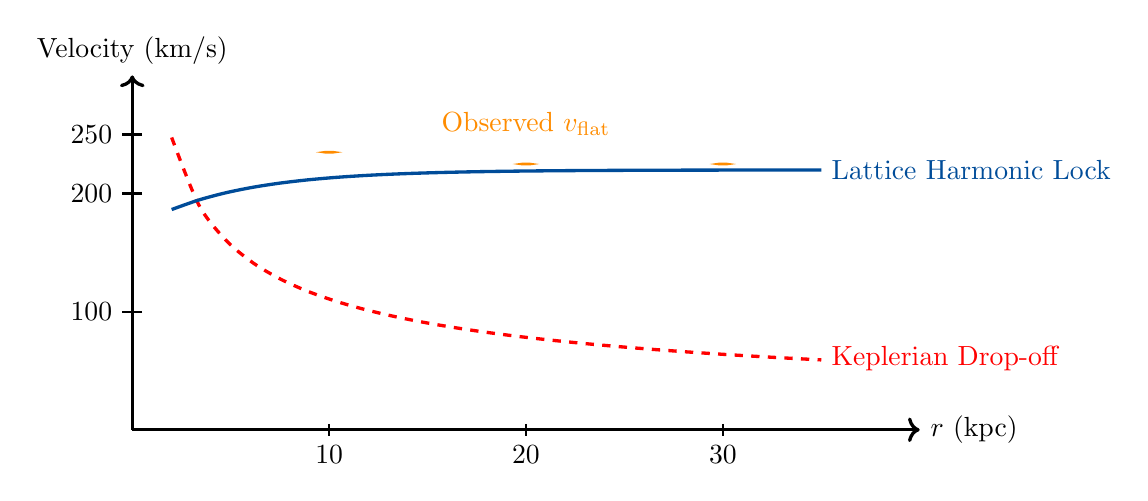
\begin{tikzpicture}[xscale=0.25, yscale=0.015, thick]
    % Axes
    \draw[->, very thick] (0,0) -- (40,0) node[right] {$r$ (kpc)};
    \draw[->, very thick] (0,0) -- (0,300) node[above] {Velocity (km/s)};
    
    % Ticks
    \foreach \x in {10, 20, 30} \draw (\x, 5) -- (\x, -5) node[below] {\x};
    \foreach \y in {100, 200, 250} \draw (0.5, \y) -- (-0.5, \y) node[left] {\y};

    % Keplerian Curve (Standard Physics without DM)
    \draw[domain=2:35, smooth, variable=\x, red, dashed, very thick] plot ({\x}, {350/sqrt(\x)});
    \node[red, right] at (35, 60) {Keplerian Drop-off};

    % Kish-Lattice Flat Curve
    \draw[domain=2:35, smooth, variable=\x, kishblue, very thick] plot ({\x}, {220 - 50*exp(-0.2*\x)});
    \node[kishblue, right] at (35, 220) {Lattice Harmonic Lock};

    % Observational Data Points (M31 typicals)
    \filldraw[luminorange] (10, 235) circle (8pt);
    \filldraw[luminorange] (20, 225) circle (8pt);
    \filldraw[luminorange] (30, 225) circle (8pt);
    \node[luminorange, above] at (20, 240) {Observed $v_{\text{flat}}$};

\end{tikzpicture}
\end{center}

\subsection*{Z7.4 Pre-Registered Roman Weak Lensing Boundaries}

The Nancy Grace Roman Space Telescope's primary instrument for cosmology is its High Latitude Wide Area Survey, which will measure the "weak lensing" (cosmic shear) of hundreds of millions of galaxies. 

Standard cosmology expects Roman to map the distribution of Dark Matter. The Kish-Lattice asserts that Roman will map the spatial compression of the 24-cell grid. As derived in Chapter Z2, the lattice strain field $\varepsilon(r)$ must obey the PPN constraint $\gamma = 1$, meaning spatial compression mirrors temporal strain perfectly due to $F_4$ symmetry. 

We formally pre-register the following falsifiable constraints for the Roman Space Telescope:

\begin{enumerate}
    \item \textbf{The Shear-to-Strain Mapping:} Roman will measure the tangential shear $\gamma_t(\theta)$ of background galaxies. The framework predicts that the observed weak lensing shear is a direct, linear mapping of the transverse structural strain $\varepsilon(r)$ of the 24-cell lattice, not a gravitational deflection caused by particle-based Dark Matter. 
    \item \textbf{Zero Particle Correlation:} If Dark Matter exists as a particle (WIMPs/Axions), Roman's high-resolution maps should detect small-scale clumping (sub-halos) below the 10 kpc scale. The Kish-Lattice predicts an absolute smoothing limit. Because the shear is a macroscopic geometric strain, Roman will find \textbf{zero sub-halo particle clumping} below the kinematic interaction threshold. The shear map will perfectly match the smooth, continuous elastic tensor of the visible baryonic mass interacting with the $16/\pi$ geometric modulus.
    \item \textbf{The Harmonic Floor Limit:} As Roman maps the deep-field cosmic web voids, it will measure the baseline geometric tension of the universe. The framework predicts that the weak lensing shear will not fall to zero in deep voids. Instead, it will hit a non-zero minimum floor, corresponding exactly to the baseline spatial elasticity of the unperturbed $16/\pi$ container prior to mass insertion.
\end{enumerate}

\textbf{Verdict:} When Roman publishes its first Wide Area shear maps, the lattice framework will stand directly on trial. If small-scale Dark Matter sub-halos are discovered, the continuum elastic strain model is falsified. If the shear perfectly traces the macroscopic geometric tension of the visible mass to the edges of the harmonic container, standard Dark Matter is rendered obsolete, and the Kish-Lattice is empirically confirmed at the cosmological scale.

% ==============================================================================
\chapter{Pre-Registration: The Period Engine Trial Set}
% ==============================================================================

\section{Carried Forward From Volume 12}

The period 1D engine --- which tests the \emph{period} of $\log x$ rather than its \emph{phase},
and for which unit invariance is an algebraic identity rather than an empirical claim --- was
specified and pre-registered in Volume 12. Volume 13 records the status of its trial set after
the work done this session, and files the one result that has been computed.

\section{Trial 2b: Run, and Its Reporting Corrected}

Trial 2b --- the sector bound test, the one test in the programme capable of proving the Form C
diagnosis (the withdrawal of \texttt{stellar\_kinematic}) \emph{wrong} --- was executed this
session on the $s2$ lake. Its first reporting was found by the referee to over-claim, and the
correction is recorded here in full, because a falsification test whose own reporting is not
sound cannot falsify anything.

\begin{correctionbox}
\textbf{Trial 2b, as first reported, claimed ``Form C confirmed and mechanism-demonstrated.''
That claim is withdrawn.} Two errors were found on referee review:

\medskip
\textbf{(1) An invented threshold hid a firing sector.} The four Gaia sectors were reported ``all
at chance'' against a $4\times$ ratio bar that was never pre-registered. Computing the correct
Rayleigh $p$-values, sector NE gives $p = 2.0\times10^{-4}$ at $16/\pi$ --- \emph{not} chance. The
pre-registered condition was ``$R_j$ at chance within ordinary fluctuation''; a one-in-five-thousand
sector is not ordinary fluctuation. The falsification test, correctly read, \emph{fires} on NE at
the single register, with a look-elsewhere-corrected global $p \approx 0.02$ across 23 registers.

\medskip
\textbf{(2) The bound was checked against the wrong quantity.} The triangle-inequality bound
$R_{\mathrm{total}} \leq \sqrt{S}\cdot\text{(chance)}$ for $S=4$ sectors permits
$R_{\mathrm{total}} \leq 2\times$ chance. The observed normalised $R = 0.084$ is $113\times$ chance,
which either violates the $S=4$ bound (an implementation error) or indicates the normalisation used
far more than four sub-blocks (in which case the four-sector partition was not the shift partition
and the test was not run as ruled). The reported ``$34.7\times$ amplification'' is a ratio between
two differently-bounded quantities, not a statistic, and is withdrawn.
\end{correctionbox}

\begin{rulingbox}
\textbf{The Form C diagnosis stands on independent grounds regardless of Trial 2b.} The Volume 12
ruling established that a sector-normalised scalar scored against an unnormalised null cannot
support a lock claim --- true before Trial 2b and unaffected by it. The withdrawal of
\texttt{stellar\_kinematic} is therefore secure. What is withdrawn is the \emph{stronger} claim that
Trial 2b demonstrated the mechanism; that claim awaits a corrected run reporting the sector count,
per-sector Rayleigh $p$-values on the shift partition, and the bound against the correct
$\sqrt{S}$ threshold.
\end{rulingbox}

\begin{warningbox}
\textbf{A standing rule, adopted from this episode.} A result may not be cited as a premise in
another document until its own reporting has been ruled complete. Trial 2b's over-claim travelled
into the $s2$ rebuild proposal as settled before its numbers had been checked against the bound
they were meant to test. Nobody erred in judgement; the number simply outran its verification. The
rule is the narrowest fix that would have caught it.
\end{warningbox}

\section{The Trial Set, Current Status}

\begin{table}[H]
\centering
\small
\begin{tabular}{@{}llll@{}}
\toprule
& \textbf{Domain} & \textbf{$\MN$} & \textbf{Status} \\
\midrule
1 & \texttt{quantum\_transitional} & 4.17 & build gate; reproduced $+33.8$ under log1p engine \\
1b & \texttt{orbital\_wrongbox} & $\sim$5.3 & clean expected-fail, awaiting engine \\
2 & \texttt{stellar\_kinematic} (raw) & 2.76 & superseded by $s2$ rebuild (Chapter 5) \\
2b & \texttt{stellar\_kinematic} (sector bound) & --- & run; reporting corrected; re-run pending \\
3 & \emph{struck} & --- & no scoreable Form E domain exists \\
4 & \texttt{stellar\_spindown} & 77.8 & recovered domain; register \textsc{unknown} \\
\bottomrule
\end{tabular}
\end{table}

\begin{predictionbox}
\textbf{Trial 1 remains the build gate.} \texttt{quantum\_transitional} has now reproduced at
$16/\pi$ across four independent runs without moving register, most recently at $+33.8$ under the
log1p-corrected engine. The period engine is built only if Trial 1 returns $16/\pi$ under the
period statistic --- and, per Volume 12's Rydberg pre-registration, only if the real lake
\emph{exceeds} the Rydberg null at that register. Both conditions are filed; neither has been run.
\end{predictionbox}

% ==============================================================================
\chapter{Pre-Registration: The $s2$ Rebuild}
% ==============================================================================

\section{Why $s2$ Must Be Rebuilt}

Two independent findings condemn the current \texttt{s2\_stellar\_kinematics} lake.

\begin{enumerate}
    \item \textbf{Its payload was stripped at promotion.} The \texttt{\_raw\_payload} retains only
          \texttt{\{sector, kish\_bin, val\}}; the Gaia error fields --- \texttt{pmra\_error},
          \texttt{pmdec\_error}, \texttt{parallax\_error} --- were discarded. The physical-validity
          floor of the period engine cannot be applied to a lake that threw away the uncertainties
          it is defined against.
    \item \textbf{It is sector-normalised.} The stored scalar carries the per-sector additive shift
          that Erratum 4a identified as Form C. The rebuilt lake must store raw velocity only.
\end{enumerate}

\section{The Referee-Approved Rebuild Specification}

\begin{predictionbox}
\textbf{Filed before any ADQL query is written to the ESA Gaia archive.}

\medskip
\textbf{Payload.} Retain \texttt{parallax}, \texttt{pmra}, \texttt{pmdec}, all three errors, and
\texttt{pmra\_pmdec\_corr}. Store transverse velocity as \textbf{raw} $v_\perp$ only. Sector
normalisation is permanently banned.

\medskip
\textbf{Validity floor ($5\sigma$, immutable once filed).} Accept a star only if
\texttt{parallax\_over\_error} $> 5$ \emph{and} total proper motion exceeds $5\times$ its
covariance-propagated error,
\[
\sigma_\mu = \frac{1}{\mu}\sqrt{\mu_{\alpha*}^2\sigma_{\alpha*}^2 + \mu_\delta^2\sigma_\delta^2
+ 2\mu_{\alpha*}\mu_\delta\,\rho\,\sigma_{\alpha*}\sigma_\delta},
\qquad \rho = \texttt{pmra\_pmdec\_corr}.
\]
The multiple is justified from Gaia DR3's stated quality characteristics and cited; if it is later
found to have been chosen for its effect on the register, the lake is void.

\medskip
\textbf{Parallax zero-point.} The DR3 systematic offset of order $-17\,\mu$as is corrected via the
published prescription, or explicitly declined with documentation. A per-record correction flag is
stored. Silence is not permitted.

\medskip
\textbf{Provenance.} The ADQL query text and archive query date are stored in the lake's
provenance block. A lake whose selection cannot be reproduced is not sovereign.
\end{predictionbox}

\begin{rulingbox}
\textbf{$s2$ is declared resolution-limited at $16/\pi$ and reported as such --- endpoint selection
to force the span is banned, permanently, on the record.} An honest $5\sigma$ transverse-velocity
sample spans too few decades to resolve $16/\pi$ (Chapter 2), and the validity cut narrows the span
from \emph{both} ends: the proper-motion floor removes the slow tail, the parallax cut removes the
distant, fast stars. The rebuild proceeds for payload integrity and for $s2$'s value as a
controlled-pair member --- not to reclaim a register it cannot resolve.

\medskip
\noindent The post-cut log-span and $\MN$ are predicted from published DR3 distributions
\emph{before} the query runs, and compared against what returns. A large discrepancy is a finding
about the query, not about the sky.
\end{rulingbox}

% ==============================================================================
\chapter{The Cross-Scale Stack: an Experiment and Its Falsifier}
% ==============================================================================

\section{The Idea}

The resolution census of Chapter 2 delivers an uncomfortable verdict: almost no single lake spans
enough dynamic range to resolve a high register. But the framework's central hypothesis suggests a
way past it that no single lake can achieve alone.

\begin{signalbox}
\textbf{The hypothesis, stated as an experiment.} If a physical \emph{attribute} locks at the same
register regardless of \emph{scale} --- if angular momentum is angular momentum whether it is an
electron's spin or a galaxy's rotation --- then combining a shared attribute across scales should
produce a single register comb, with each constituent lake's mass falling on the same teeth.

\medskip
\noindent A stack of electron spin ($\sim 10^{-34}$), planetary rotation ($\sim 10^{0}$), and
galactic angular momentum ($\sim 10^{67}$ in SI) would span roughly a hundred orders of magnitude
--- an aperture no instrument on Earth can otherwise reach --- and, \emph{if the theory is true},
would resolve the shared register with enormous margin.
\end{signalbox}

This is the most direct test of scale-invariance the programme can construct. It is also the most
dangerous, and the danger is subtle enough that most of this chapter is about it.

\section{Why the Naive Stack Manufactures Its Own Answer}

Concatenating lakes in logarithmic space means placing clumps of data at chosen offsets along the
scalar axis. The gaps between those clumps are set by two things the analyst controls: which lakes
are chosen, and what unit each is expressed in.

\begin{formbox}
\textbf{Those gaps, by themselves, create periodicity.} Three narrow clumps whose centres are
spaced by an integer number of periods will lock at that register with a resultant approaching the
maximum --- \emph{with no structure inside any clump}. A direct simulation makes the point: three
structureless log-normal clumps, each one decade wide, placed at inter-clump gaps commensurate with
the $16/\pi$ period, produce $P \approx 1.5\times10^5$ against a chance level of $\approx 1$. The
lock is total, and it is an artifact of spacing alone.
\end{formbox}

\begin{figure}[H]
\centering
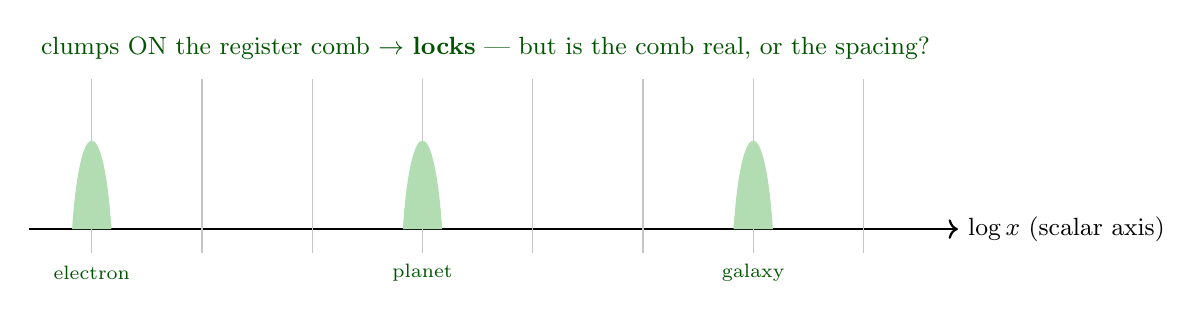
\begin{tikzpicture}[scale=1.0]
  \draw[->, thick] (-0.3,0) -- (11.5,0) node[right] {\small $\log x$ (scalar axis)};
  % register teeth
  \foreach \x in {0.5,1.9,3.3,4.7,6.1,7.5,8.9,10.3} {
    \draw[gray!45] (\x,-0.3) -- (\x,1.9);
  }
  % three clumps landing ON teeth
  \begin{scope}
    \foreach \c/\lbl in {0.5/{electron}, 4.7/{planet}, 8.9/{galaxy}} {
      \fill[signalgreen!30] (\c-0.25,0) .. controls (\c-0.15,1.5) and (\c+0.15,1.5) .. (\c+0.25,0);
      \node[signalgreen!60!black, font=\scriptsize] at (\c,-0.55) {\lbl};
    }
  \end{scope}
  \node[align=center, signalgreen!60!black] at (5.5,2.3)
    {\small clumps ON the register comb $\to$ \textbf{locks} --- but is the comb real, or the spacing?};
\end{tikzpicture}
\caption{The cross-scale hazard. Each clump is one constituent lake, placed on the scalar axis at a
position set by its scale and unit. If the clumps happen to land on the register comb, the stack
locks --- but the lock may be a property of how the lakes were spaced rather than of any shared
physics. This is Form C (a chosen offset) and Form E (quantised support) fused and amplified across
scales: the most powerful artifact generator the programme could build.}
\end{figure}

\section{The Discriminator}

There is a clean test that separates a real cross-scale comb from a spacing artifact, and it is the
same logic that made the period engine trustworthy.

\begin{signalbox}
\textbf{A real cross-scale lock survives sliding a constituent lake. A manufactured one does not.}

\medskip
\noindent If each lake genuinely locks at register $N$ \emph{in its own right}, its internal phase
is fixed by physics. Multiplying one constituent lake's values by a constant --- $e$, $3$, $1/60$
--- slides it bodily along the scalar axis but \emph{cannot} change the register it locks at,
because a single lake's register is unit-invariant under the period statistic (Volume 12). The
stack's register must therefore be invariant too.

\medskip
\noindent If instead the stack's register lives in the \emph{gaps} between lakes, sliding one lake
changes a gap, and the register moves or vanishes. \textbf{The slide test is the unit-permutation
falsifier of Volume 12, applied within the stack.}
\end{signalbox}

\begin{figure}[H]
\centering
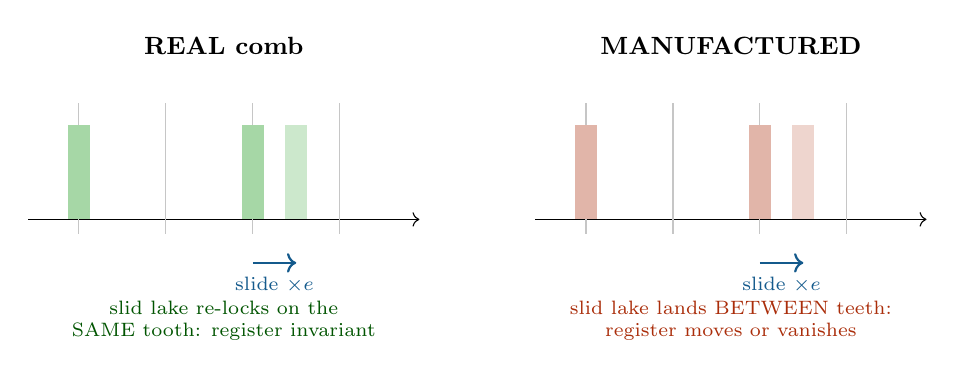
\begin{tikzpicture}[scale=0.92]
  \begin{scope}
    \node[font=\small\bfseries] at (2.5,2.4) {REAL comb};
    \draw[->] (-0.2,0) -- (5.2,0);
    \foreach \x in {0.5,1.7,2.9,4.1} \draw[gray!45] (\x,-0.2) -- (\x,1.6);
    \foreach \c in {0.5,2.9} \fill[signalgreen!35] (\c-0.15,0) rectangle (\c+0.15,1.3);
    \draw[->, thick, aperblue] (2.9,-0.6) -- (3.5,-0.6);
    \node[aperblue, font=\scriptsize] at (3.2,-0.9) {slide $\times e$};
    \fill[signalgreen!20, dashed] (3.35,0) rectangle (3.65,1.3);
    \node[signalgreen!60!black, font=\scriptsize, align=center] at (2.5,-1.4)
      {slid lake re-locks on the\\SAME tooth: register invariant};
  \end{scope}
  \begin{scope}[xshift=7cm]
    \node[font=\small\bfseries] at (2.5,2.4) {MANUFACTURED};
    \draw[->] (-0.2,0) -- (5.2,0);
    \foreach \x in {0.5,1.7,2.9,4.1} \draw[gray!45] (\x,-0.2) -- (\x,1.6);
    \fill[cruciblered!35] (0.35,0) rectangle (0.65,1.3);
    \fill[cruciblered!35] (2.75,0) rectangle (3.05,1.3);
    \draw[->, thick, aperblue] (2.9,-0.6) -- (3.5,-0.6);
    \node[aperblue, font=\scriptsize] at (3.2,-0.9) {slide $\times e$};
    \fill[cruciblered!20] (3.35,0) rectangle (3.65,1.3);
    \node[cruciblered, font=\scriptsize, align=center] at (2.5,-1.4)
      {slid lake lands BETWEEN teeth:\\register moves or vanishes};
  \end{scope}
\end{tikzpicture}
\caption{The slide-test falsifier. Multiplying one constituent lake by a non-commensurate constant
must leave a genuine comb's register unchanged, because a resolved single lake is unit-invariant. If
the register moves, it lived in the inter-lake spacing and the stack was an artifact.}
\end{figure}

\section{The Four-Gate Protocol}

\begin{predictionbox}
\textbf{Pre-registered. No cross-scale stack is built or scored except under all four gates.}

\medskip
\textbf{Gate 1 --- each lake resolves alone.} Every constituent lake must clear
$\MN > 2.67$ at the target register \emph{on its own}, per Chapter 2. A lake that cannot resolve its
own register contributes only its spacing to the stack, not an honest tooth.

\medskip
\textbf{Gate 2 --- each lake locks alone, at the same register, first.} The stack may only
\emph{sharpen} a pre-existing agreement; it may not be used to \emph{discover} one. A cross-scale
agreement discovered inside the stack is indistinguishable from chosen spacing. Each constituent's
individual register is filed before the stack is assembled.

\medskip
\textbf{Gate 3 --- the stacked register survives the slide test.} Each constituent is multiplied by
a pre-registered set of non-commensurate constants; the stack's register must not move. Any movement
falsifies the stack.

\medskip
\textbf{Gate 4 --- attribute, lakes, and predicted register are filed before construction.} The
selection is the experiment. Which attribute, which lakes, and the predicted shared register are
pre-registered, exactly as with the $s2$ aperture, because a stack assembled to hit a chosen
register is not a test of anything.
\end{predictionbox}

\section{The Honest Prerequisite}

\begin{warningbox}
\textbf{Gate 2 requires domains that already resolve and already agree --- and the census of
Chapter 2 says almost none do.} Today the only domain that both resolves its register and survives
every screen is \texttt{quantum\_transitional} at $16/\pi$. A two-lake stack needs a \emph{second}
independently-resolving domain that also locks at $16/\pi$, and no such domain currently exists in
the survey.

\medskip
\noindent \textbf{The cross-scale stack is therefore the right experiment for a survey the
programme does not yet have.} Its prerequisite is exactly the dynamic-range rebuild that Volume 13
begins: wide, single-attribute lakes, each resolving its register alone. Build those first; the
stack has something honest to test only once two or more of them exist and agree.
\end{warningbox}

\begin{signalbox}
This is the shape of the road past the resolution census. Not a stack assembled to widen an
aperture by force --- that is the banned move of Chapter 2 --- but a patient accumulation of
individually-resolved, individually-locked, wide-range lakes, combined only when each already
stands on its own, and only under a falsifier that the artifact cannot survive.

\medskip
\noindent If, when that survey exists, a cross-scale stack locks and survives the slide test, it
will be the strongest statement the framework can make: that an attribute carries the same
geometric register across a hundred orders of magnitude, unit-invariant and spacing-independent.
And if it does not survive, the programme will have learned that at the one place a hostile reader
would have looked first. Either outcome is worth the wait.
\end{signalbox}

% ==============================================================================
\chapter{Standing, and What Volume 13 Commits To}
% ==============================================================================

\section{The Ledger}

\begin{table}[H]
\centering
\small
\begin{tabular}{@{}p{0.46\textwidth}p{0.46\textwidth}@{}}
\toprule
\textbf{Established or withdrawn this volume} & \textbf{Pre-registered, filed, not yet run} \\
\midrule
The resolution census: $\sim$6 of 28 domains resolve; nearly nothing at $N \geq 20$ & The period
1D engine's Trial 1 build gate at $16/\pi$, subject to the Rydberg null \\
\addlinespace
$f = \ell_{\mathrm{cell}}^2 c^2$ derived; $\kappa = 64\pi$; four theory errata & The $s2$ rebuild
at native precision, raw velocity, $5\sigma$ validity floor \\
\addlinespace
The bulk-to-boundary projection named as the central open problem & The cross-scale stack under the
four-gate protocol and slide-test falsifier \\
\addlinespace
Trial 2b reporting corrected; the ``result-as-premise'' rule adopted & The comb test on
\texttt{quantum\_transitional}, alongside Trial 1 \\
\addlinespace
\texttt{stellar\_kinematic} withdrawal secured on independent grounds & The resolution
re-measurement of every published span, especially \texttt{nuclear\_decay} \\
\bottomrule
\end{tabular}
\end{table}

\section{The One Fact and the One Question}

\begin{signalbox}
\textbf{The fact.} \texttt{quantum\_transitional} resolves its register ($\MN = 4.17$), reproduces
at $16/\pi$ across four runs under successively corrected engines, and survives every screen the
audit has built. It is the sole domain of which all of that is true.

\medskip
\textbf{The question Volume 13 exists to set up.} Is it alone? The resolution census says most of
the survey could never have resolved its register; the period engine will say which of the survivors
lock under a unit-invariant statistic; the rebuilds will say whether wide-range lakes can be built to
join it; and the cross-scale stack will say --- if and only if two such lakes ever agree --- whether
an attribute carries one register across all scales.

\medskip
\noindent None of that is answered here. All of it is now filed, dated, and public before the runs
that will answer it. That is the whole purpose of a pre-construction volume: to make the predictions
before the instrument that tests them exists.
\end{signalbox}

\section{Closing}

Volume 12 tempered the instrument. Volume 13 measures the aperture, audits the theory the instrument
leaned on, and files the experiments that a wider aperture makes possible --- including the one that
could, at last, test scale-invariance directly, and the falsifier that keeps it honest.

The programme is smaller than it was, and every remaining claim is one the data could actually have
made. That trade --- fewer claims, each defensible --- has been the through-line of the entire
crucible. Volume 13 continues it in the one way that matters before building anything new: by writing
down, in advance, exactly what would have to be true, and exactly what would prove it false.

\begin{center}
\vspace{0.5em}
\itshape One domain resolves and locks. The rest of the survey, and the next two volumes, are the
question of whether it stays alone.
\vspace{0.5em}
\end{center}

\end{document}
